\documentclass[12pt, letterpaper]{article}
\usepackage[margin=1in]{geometry}
\usepackage{graphicx}
\usepackage{amsmath}
\usepackage{amssymb}
\usepackage{tikz}
\usepackage{hyperref}
\hypersetup{
	colorlinks = true,
	linkcolor = black,
	urlcolor = blue
}

\title{
	{GV100 Intro to PolTheory}\\
	{\large{Professor Katrin Flikschuh}}\\
	{\large{Essay Plan Document}}
}
\author{Cedric Tan}
\date{April 2019}

\begin{document}
\maketitle
\begin{abstract}

This is a construction of some essay plans for MT and LT topics from the Introduction to Political Theory Module. Essay plans are sparse throughout the document and can be found at the end of \textbf{parts} of each thinker. If they are longer, that means more time has been dedicated to them due to particular interest. The notes are mine fully and may not be authentic to the lecturer's as they have been modified.

The format of this material is usually recounted lecture by lecture, which is to say a week by week recount. Material may be merged together as it fits appropriately with one another such as multiple weeks on the same thinker.
\end{abstract}
\newpage
\tableofcontents
\newpage

\section{Plato}
We will begin with a recap on Plato's main ideas before moving onto essay constructions. This section is split into two parts, the first concerning \textbf{Plato and Justice} and the second concerning \textbf{Plato and his Preservation of Justice.}
\subsection{Part 1: Plato and Justice}
Plato's motivation is to find the just city and to figure out what the just city entails. 
\subsubsection{Plato and Thrasymachus}
We begin with the dialogue between Plato and Thrasymachus. Platonic justice is \textbf{unknown in the beginning,} what we do have is a conception of Thrasymachean Justice:
\begin{itemize}
	\item Whatever is right for the stronger
	\item To the advantage of the stronger
\end{itemize}
However, even with Thrasymachus we are unsure about his motivations for justice. Are they \textbf{factual i.e. descriptive} or are they \textbf{normative i.e. what we should strive to do?} He could be advertising both in his theory, which is perfectly acceptable. Despite this, Plato is unsatisfied with Thrasymachus' conclusion. Injustice produces faction and hatred. For Plato, this means that the soul is ultimately unbalanced.

\subsubsection{Characteristics of Justice}
For Plato, there are certain characteristics that must be inherent in justice: 
\begin{enumerate}
	\item There needs to be a desirability of justice so as to make people act in a justifiable manner without the need for coercion
	\item Justice must be a good in itself, this means that it isn't a means to an ends, good or bad, but rather the idea of justice is itself good. The products of justice do not matter in this discussion. However, if justice is a good in itself, it should follow that its products are good too
	\item Justice is also the excellence of the soul which means that the soul is harmonious in a metaphysical sense
	\item Justice also has positive effects on other people, referencing point 2
\end{enumerate}

\subsubsection{Conventional and Platonic Justice}
Thus, moving on from its characteristics, we can argue that types of justice may appear to have these characteristics so we need to ensure that we can distinguish these \textbf{conventional} forms of justice from our \textbf{Platonic} form.
\begin{itemize}
	\item Conventional $\rightarrow$ justice in terms of appearance and practice
	\item Platonic $\rightarrow$ justice as a good in itself in an idealistic form
\end{itemize}
So, the confusion can be illustrated as follows:
\begin{center}
	\noindent\fbox{\begin{minipage}{.9\textwidth}
	Take the characteristics of \textbf{intelligence} and \textbf{courage.} Now, let's compare these characteristics, respectively, to \textbf{slyness} and \textbf{cunning.} Here, we can see that these characteristics have some similar traits and can be conflated at times. Yet, the latter traits are seen to have unjust motivations. This is the concern when attempting to distinguish between \textbf{Conventional} and \textbf{Platonic} forms of justice.
	\end{minipage}}
\end{center}
To add further complication to this matter. There are motives to be just without a harmonious soul, hence, again, on appearance we might look just but the motivations are simply not in the right order. A key exmaple of this would be \textbf{Hobbesian fear of punishment} as you act in a just manner to obtain security rather than \textit{acting for justice itself,} which is what Plato says is the important thing to do.

Hence, it is \textbf{very difficult to distinguish} between the two as, on the surface, they look as if they are the same thing entirely.


\subsection{Part 1: Study Questions and Plans}
Below are study questions and short, planned responses to them.
\subsubsection{Thrasymachus}
\textbf{Question:} How does Thrasymachus defend his claims? Are his arguments convincing?\\\\
We begin by understand Thrasymachus' claims:
\begin{itemize}
	\item Justice is whatever is good for the stronger
	\item Where the power lies is where justice lies $\rightarrow$ governments, democratic, tyrannical and so on, make laws which are specific and to the benefit of their government type, hence their actions are just
	\item The subjects in these governments are to follow these laws and rules to the benefit of their government type, if they act accordingly, they are labelled as just
	\item Justice is obedience to laws
	\item Justice is nothing but the advantage of another
\end{itemize}
\textbf{Arguments}\\
This is, on face value, a very attractive conception of justice. We conform to a system of rules created by people in power and believe in them because they hold us and everyone else accountable to the system whilst making the system itself function. Hence, it would seem convincing, in a rather cynical sense, that we are weak people following the rule of those who dictate and just have the \textbf{belief that what we are doing is considered just.}

This idea is just as plausible today as it was with Thrasymachus. Think about big government in places such as Russia (less so) or North Korea, the subjects in those countries believe their actions are just as long as they conform to the set of rules laid out. Subjects are literally strong-manned into conforming to that system of 'justice'.

Thus, this means that the subjects, from Thrasymachus point of view, are seen to be just while \textbf{the rulers who take advantage of their just behaviour are seen to be unjust.} Thrasymachus goes onto list various examples of where the just are far worse off than the unjust. The first example he uses is the idea of \textbf{contracts} $\rightarrow$ where the unjust person will leave better off than the unjust due to some abuse of the contract that the unjust person is willing to commit that the just person would not.

Further, the idea of \textbf{justice as nothing but the advantage of another} advocates some sort of ethical egoism. This argument, again from a cynical point of view, seems to work out. However, to prescribe egoism is a difficult task and if attacking Thrasymachus from this point of view, it would be easy to pick apart his argument. Let us not take this argument with as much weight to be charitable to his other arguments. \\\\
\textbf{Counter-arguments}\\
For Plato, this seems questionable and concerning for a few reasons:

One of them is because of the fact that even rulers are \textbf{fallible,} which means that they themselves are prone to making mistakes. If subjects, willing to be just, aim to conform to the ruler's specifications at all times, then when rulers incorrectly institute a law that is not in their advantage, we find ourselves in a self-contradicting situation whereby the just subjects, in their attempts to be just, \textbf{are acting to the disadvantage of the stronger,} despite the stronger instituting said laws. This means that \textbf{obedience is occasionally not in the interests of the stronger.} The issue that Plato must face is Thrasymachus' claims that \textbf{rulers who do not act in their own advantage are not effectively ruling.} However, this claim seems to be absurd in the sense that ruling is a continuous activity and if we were to segment it into successes and failures in ruling, it would seem that the ruler has not ruled continuously at all.

Another is Plato's concern with the soul and its excellence. If we are to simply look at justice as the advantage of the stronger, it might not be the case that our soul is harmonious at all. Taking the unjust argument from Thrasymachus, where the unjust man is always better off than the just, we recognise the possibility that under the Thrasymachean system, we are approaching justice in a strictly conventional manner rather than a Platonic manner, hence Plato's dissatisfaction.  \\\\
\textbf{Evaluation}\\
Are Plato's arguments against Thrasymachus satisfactory? To a certain extent, they seem to be. The argument from self-contradiction appears to defeat the Thrasymachus' initial argument and further, the harmonious excellence of the soul which is emphasised in the Platonic doctrine has its merits.

Yet, this still does not account for the skeptic, that justice which surrounds us is purely conventional and that the idealistic conception of justice makes no sense to adopt because of its very idealistic nature. If we take the material perspective, that is, to disregard all idealistic conceptions, we might have to give Thrasymachus a lot more credit than he is given.

Thus the side of the argument you take is entirely dependent on your world-view. If you think that the conventional justice really \textbf{is not justice at all} and that an idealistic justice is the only form of justice that is truly \textit{justified} then you are able to disregard the Thrasymachean argument. Yet, in a very \textbf{practical sense,} it would seem that Thrasymachus appears to tap into our doubts of the very systems in which we live.

\subsubsection{Soul and City, an analogy}
\textbf{Question:} Towards the end of Book 1, Plato has Socrates introduce an analogy between 'justice as a virtue of the soul' and 'justice as a virtue of the well-ordered polis.' Why does he draw this analogy? Is the idea that the just polis is comparable to the just person? Or is the thought, rather, that for a just polis to be possible, we have to have just persons?\\\\
We begin by understanding the two analogies that Socrates puts together. Below are both the \textbf{Soul} and the \textbf{City} with their \textbf{constituent parts.}
\begin{center}
	\begin{tabular}{c|c}
		\textbf{Soul} & \textbf{City}\\
		\hline
		Appetites & Artisans\\
		\hline
		Spirit & Guardians (Auxiliaries)\\
		\hline
		Reason & Philosopher Kings\\
		\hline
	\end{tabular}
\end{center}
Here is a refresher on the roles of each:
\begin{itemize}
	\item Appetites or the Artisans $\rightarrow$ here to meet our daily needs and bodily well-being
	\item Spirit or the Guardians $\rightarrow$ here to give us our intuitive guidance and establish our virtues as people or as a city
	\item Reason or the Philosopher Kings $\rightarrow$ here to govern us
\end{itemize}
\textbf{Think of society as a ship at sea:}
\begin{itemize}
	\item It is dependent on who is the captain and what roles each individual has on the boat
	\item The true helmsman wants to sail smoothly and safely but still towards a set direction
	\item This can be achieved in a \textbf{just} manner
	\item Necessarily, this involves all components to be working \textbf{harmoniously}
\end{itemize}
% Underfull hbox - fix later
\textbf{Just Polis as comparable to the Just Person}\\
Recall that justice comes from the harmony of components within an entity. Plato discussed this idea with justice in an individual. This is seen through the balancing act of all components of the soul whereby if each individual component is doing its part, through the guidance of reason, which is a part in itself, we will be operating as a just person. This is because we have some necessities which are fulfilled by our appetites such as fulfilling our need to sleep or eat whilst also establishing our virtues and guidance on where to go with our spirit.

This is comparable to the just polis in a sense due to the idea of how a polis is constructed in a similar manner. Roles are given within society, that much is given. When you fulfil these roles and everyone else does the same, we will be operating as a just city due to the fact that there is a certain harmony within the city itself. This harmony subsequently means that the soul, in a sense, of the city is inevitably excellent. \\\\
\textbf{Just Polis requires Just Persons}
The second possibility of this analogy is a hint towards a political ideology of instituting a just city by creating just people. This makes intuitive sense as the requirement of harmony, to create a just city, flows easily from the individuals in said city being just. If the purpose of an individual is to fulfil a particular role in society, their spirit and reason will lead them there \textbf{on the assumption that the individual is already just.} This will lead to all roles, the artisans, guardians and philosopher kings, being fulfilled and operating at the best level they can be operating at.

Taking these factors into account, which we can label as a bottom up approach, the just individual will lead into the just city. This argument is strong because it does not leave out any individual in the polis whatsoever. It appears that it is a necessary requirement for all individuals in the polis to be just for the polis itself to be just. \\\\
\textbf{Evaluation on analogies}\\
The \textbf{first argument,} a comparison of the soul to the city, appears to be approachable in a strictly functionalist sense. If all constituent parts of the soul, like all constituent parts of the city, are working strictly by their function, we can see that the argument makes sense. From that point of view, the analogy makes some sort of sense.

Yet, it would be hard-pressed to say that the constitution of one person's soul is the same as the constitution of a city. The plethora of moving parts that exist in an operating polis seems to be incomparable or reducible to the three components of the soul. Within the Artisan class, for example, a great number of artisan crafts exist which might all have different idealistic purposes and so on. Hence, from a practical sense, the idea seems absurd to compare the two (Ferrari 2003). Further, could they be mutually exclusive? If I aimed to maintain a harmonious soul, could I still fulfil my function? Perhaps not, and if that is the case, then it'd be unlikely for a just individual to live in a just polis.

Does this take away from the strength of the analogy though? If the practicality is such that it is not only function that is required to be fulfilled, it might diminish Plato's argument. However, the simplistic nature of the analogy makes the argument approachable and sensible in a clarified manner. It makes sense that for a city to be just, its internal gears all need to be operating smoothly in some manner.

The \textbf{second argument,} just individuals leading into a just city, is convincing to a large extent because of this bottom-up approach that I had touched on. By necessarily requiring all individuals to be just to constitute a just city, we nail down the functionality argument along with the harmonious and excellence requirement from the get go. Thus, it would make a lot of sense to start a city, with the aim for it to be just, if we have just individuals founding it.

Yet, we have a \textbf{chicken and egg problem} because although we would love to nail down these requirements initially, it seems idealistic to believe all individuals will be just before founding the city. It would seem more plausible to have a just city, more or less, that trains people to be just. But then again, who would constitute that just city? Perhaps we can reduce the requirements for the creation of a just city by having \textbf{some just individuals} instead of them all being just. That's a point of contention that might need to be studied further.

\subsubsection{Arguments to Remember}
Below are some arguments to remember as reasons to be just or reasons as to why justice is preferred to injustice:
\begin{enumerate}
	\item Argument of Craft
	\item Argument from Ignorance
	\item Argument from Happiness
\end{enumerate}
\textbf{Argument of Craft}\\
The basic premise of this argument is related to ruling for the ruled or ruling for some other gain. Plato draws this analogy: there is a distinction to be made between \textbf{shepherding} and \textbf{shepherding for money.} The function of the shepherd is to shepherd the sheep and that is intrinsic to the activity, the profitability that arises from shepherding is not part of the function but just a (positive) side-effect of it.

Hence, every activity has some sort of intrinsic function that is tied to it which is found in its own objective nature. This function is not set by the agent but found in Plato's forms. Hence, \textbf{ruling is misunderstood if they do not rule for the benefit of the ruled.} Plato believes that this is the \textbf{objective function} of ruling as an activity.\\\\
\textbf{Argument from Ignorance}\\
This argument discusses how the unjust are not better off than the just. This is because a just person \textbf{wants to be better than an unjust person} but \textbf{does not want to be better than another just person.} Meanwhile, an unjust person \textbf{wants to be better than all other persons.}

Plato believes that no-one who properly understands a given practice wants to exceed another who also properly understands it. Think of a baker, if they have perfected the craft to the point where there is nothing else to learn then why would they attempt to outdo another who is at the same point as them? Hence, the excesses in the practice of justice shows ignorance of what practising justice means. These excesses are seen through those who are unjust.\\\\
\textbf{Argument from Happiness}\\
The unjust are not happier, Plato argues, as they have factionalised souls. A soul which has factions is unhappy from a Platonic point of view because of this lack of harmony that is require for a soul to be excellent and subsequently happy.

\subsection{Part 1: Appendix}
Here are some additional resources to aid revision:
\begin{itemize}
	\item \href{https://plato.stanford.edu/entries/plato-ethics-politics/#PoliPartOneIdeaCons}{Plato's Ethics and Politics in the Republic}
\end{itemize}

\subsection{Part 2: Preservation of Justice}
This part will begin to explore the institutions and systems that are required to create a just city. Below are some key ideas to remember when discussing Plato's construction and the subsequent preservation of justice:
\begin{itemize}
	\item Craft Analogy $\rightarrow$ stating that each individual has a soul which is assigned to a specific purpose
	\item Censorship $\rightarrow$ to maintain the craft analogy
	\item Abolishing private property $\rightarrow$ reducing faction and promoting cooperation for the guardians and philosopher kings especially
	\item Rigged Lotteries $\rightarrow$ placing blame on chance rather than regulation or legislation
\end{itemize}
From these ideas, one can begin to see an almost tyrannical twist to Plato's thinking.

\subsubsection{Craft Analogy}
This section will focus specifically on Plato's craft analogy. Again we revisit the three types of citizen that can be found in the just polis, \textbf{Kallipolis,} and Plato's assignment of the value of their soul:
\begin{center}
	\begin{tabular}{c|c}
		\textbf{Function} & \textbf{Value of their Soul}\\
		\hline
		Artisan & Bronze\\
		\hline
		Guardian & Silver\\
		\hline
		Philosopher King & Gold\\
		\hline
	\end{tabular}
\end{center}
Hence, when you are born, your soul is seen to be of one particular type of value and that part of your nature is immutable and objective. However, having parents of a particular soul type \textbf{does not exclude the possibility of giving birth to a different soul type.} Artisans can give birth to potential philosopher kings whilst philosopher kings can give birth to potential artisans.

The craft analogy is adopted to ensure that a role is assigned to each individual and each individual is properly trained to fulfil that role. Again, recognise that this is important for the harmonious excellence that a city requires for it to be just.

\subsubsection{Censorship}
Plato discusses various forms of censorship throughout \textbf{\textit{The Republic.}} Some common examples are listed below:
\begin{itemize}
	\item Poetry is limited so as to not provide stories that appear to be fake or dull the mind
	\item Music is limited so as to not provide sounds that dull the senses and ease individuals into a sense of complacency
	\item Authors and Poets of fiction can also be expunged if the need is felt (Books 3 and 8)
\end{itemize}
Again, censorship is here to ensure that all individuals maintain a strict adherence to the roles that they are given through the craft analogy. Hence, censorship is used to maintain the analogy from the educational stage such that this idea of purpose and adherence is driven into each individual's system. This is to ensure the excellence of a just city that Plato desires to be constantly maintained.

\subsubsection{Private Property}
Plato removes private property within the polis when training the philosopher kings and guardian class. Again, the premise of this removal is to provide a preemptive measure to faction that might occur. The premise of private property is that it defines property as excludable and rivalrous, if we take this into account, then when private property is created and taken by individuals, the contest for private property may, itself, lead to faction. Hence, to reduce disagreement or avoid it entirely and to maintain the concept of harmony and excellence, Plato takes the whole concept of private property away.

\subsubsection{Rigged Lotteries}
Another form of maintaining harmony is to ensure that people believe all that happens is up to chance. Hence, the use of rigged lotteries to dictate the allocation of resources and allocation of titles and so on is a disguise for the reality of the rulers controlling all facets of society.

\subsubsection{Why Reason?}
From the arguments above, we get the sense that the use of reason is what dictates a lot of these motives to be harmonious and strive for excellence and justice. Although it might seem intuitive for reason to rule, simply because it strives to take the best course of action, I will list below some of the reasons as to why we should not allow \textbf{appetite} and even \textbf{spirit} to \textit{take charge.}\\\\
\textbf{Appetite}\\
The issues with appetite involve always looking for more than what they already have. The fact that the appetitive part, without reason and spirit to guide it, is always hungry shows a \textbf{lack of control} and perhaps a desire to work towards \textbf{personal gain.} This is compounded by its instinctive nature which involves \textbf{no planning ahead} with it also being \textbf{heavily reactionary.} Thus, the appetitive part of the soul suffers from a short-termism and a \textbf{prioritisation of instant gratification.} Here are some examples of appetite in power:
\begin{itemize}
	\item Zimbabwe's Mugabe and appetite for power
	\item Malaysia's Najib and appetite for gain leading to corruption and kleptomancy
\end{itemize}
\textbf{Spirit}\\
The issues with spirit might not be as intuitive since the spirited part of our souls provide us with virtues and values and an instinctive guidance. However, it is the case that sometimes these values and virtues can be taken too far. If there is no restraint put on spirits worldview by reason, we can see the values that, taken too far, to be dangerous. Further, \textbf{spirit is restless} and has no limitations if taking charge, it does not care for appetite or reason and only for its \textbf{ideology.} Here are some examples of ideology that has been taken too far:
\begin{itemize}
	\item Hitler and Nazism
	\item Mao and his yellow army
	\item Stalin and his Soviet dream
\end{itemize}

\subsection{Part 2: Study Questions and Plans}
Below are study questions and short, planned responses to them:

\subsubsection{Classes of Citizen}
\textbf{Question:} Why does Plato distinguish between 3 classes of citizens?\\\\
The main argument to approach this question with is the argument from function. As we have described above, adherence to a function and performing the best you can at that function is what leads to a well-ordered polis. This is all in effort to maintain the harmonious soul and strive for the excellence of a just city. Below are further reasons why:
\begin{itemize}
	\item It happens to be that certain people are just born with a certain skillset that they cannot change
	\item To be unauthentic to that skillset would not be harmonious in the soul
	\item To be unauthentic would also mean that you are not fulfilling your function for the just city
	\item This function and conforming to function is a necessary condition for a just city which is related to the craft analogy
	\item Hence the distinction of classes of citizen provides a necessary structural component to Plato's city
	\item by creating this organised structure, the just city is able to operate without concessions or great faults meaning that there is more room to strive for the excellence that it pursues
\end{itemize}

\subsubsection{Philosophers and Ruling}
\textbf{Question:} Should philosophers be political rulers?\\
\textbf{n.b. This could be a thematic question and can take different forms but it is likely to be touched upon in the exam.}\\\\
First, a question must be asked on the context in which we apply this style of ruling. Plato's context would have been similar to a city state but now we have governments that encompass a more more unhomogenized group of peoples that might be more difficult to control than the city state.

Yet, a question we can also ask is \textbf{if the context even matters for philosopher kings?} Assuming that they have some sort of absolute knowledge, we can recognise their ability to provide us with a strict direction that is possibly independent of governments we have today.\\\\
\textbf{Arguments}\\
One argument for the philosopher king is based on their knowledge and, supposedly, superior understanding of political structures and frameworks. If the faith we put into their understanding is valid, and their knowledge is valid, they would be in the best place to direct how we construct our political systems. Plato's idea of the craft analogy and certain forms of censorship along with the dissolution of private property shows a, if radical, example of how a philosopher king would go about de-constructing our state and then subsequently rebuilding it for a particular purpose. This is one potential route of argument for the philosopher king.

Another is the supposedly \textbf{unbiased perspective} philosopher kings have on ruling. Due to their level of reason exceeding anyone elses, they would be in the best position to make decisions about their citizen body. Their unbiased perspective would also be implementing a just system for all parties, including themselves. If they were perfectly rational, as Plato would put it, the system, barring some major exogenous shocks, would operate smoothly. This is, perhaps, an idealistic argument for the philosopher king case.

In addition to the previous point, their level of education would usually exceed the average politician. This can be a strong case for the philosopher king, especially in our current context (April 2019), since there would be more deliberate action rather than reaction that might be put through in government. If they are in a position of power, these philosopher kings would not be playing a simple politician's game of \textbf{whoever shouts the loudest is seen as correct} but rather constructing a government that strives for the goal of excellence and justice in Platonic terms.\\\\
\textbf{Counter-arguments}\\
Theory is not practice and this shows in various contexts whereby what you think can be applied, in a structural way, cannot be applied whatsoever when you really have a practical attempt at it. Michael Ignatieff (2014), a Canadian philosopher and one-time politician, is a living example of this type of failure. Although he does mention that a certain \textbf{hubris} drove him to attempt a political campaign, he recognises that in the end, his vast knowledge of political philosophy does not apply whatsoever to the real world of politics. This is because the individuals you are catering towards are not as rational as you think and the ideas that you attempt to espouse do not come across as very valid in their eyes. Individuals are also selfish, not caring for the excellence of the polis as a whole but rather, caring for themselves first. \textbf{These are just a few examples of practicality clashing with a theoretical mindset.} This does not mean, however, that we should abandon theory entirely, just that adopting a purely rational and theoretical approach would not be so applicable in reality.

Further, a simple Machiavellian counter-argument can really augment the strength of Ignatieff's experience. As Machiavelli describes in \textbf{\textit{The Prince,}} the reality of politics is heavily decided by the force of \textbf{fortuna} which, boiled down, is simply just luck. Although you can attempt to control Fortuna with some sort of \textbf{virtú,} this set of behaviours is definitely not so related to the theoretical knowledge of Plato's Philosopher Kings. Philosophers may simply not know how to adapt to fortuna and their frameworks, which can sometimes be strict and immutable, might not be fit for the randomness of reality that Machiavelli emphasises. Although there is opportunity, politically, the Philosopher King might not make the best out of it.

Moreover, continuing the Machiavellian line of thought, \textbf{politics is more about experience rather than pure thought.} Both in a practical and perhaps intuitive sense, this makes sense as politics, as in the action of making or doing politics, is a craft and not a purely academic subject. Crafts, in this sense, require a lot of experience to be perfected and one cannot simply think their way there. Although this does not mean that Plato's Philosopher Kings are without experience, to draw that conclusion so quickly would be uncharitable and brash. Yet, the starting point of creating the just city and subsequently ruling it from a purely rational perspective would, from experience as Ignatieff puts it, lead to quite the disaster.\\\\
\textbf{Evaluation}\\
We have defined two sides of the spectrum and they have been two extreme cases:
\begin{itemize}
	\item \textbf{The Philosopher King} without any practical experience
	\item \textbf{The Real Politician} with pure experience and little knowledge
\end{itemize}
To conclude that either one is the solution would be, for lack of a better word, idiotic. Thus, framing the Philosopher King as such would not be charitable in argument either. Hence, the question is raised: could it be the case that a Philosopher King, filled with practical experience, get the best of both worlds? Here, we would be adopting a certain flexibility in the way we do politics as we are not always conforming to theoretical structures or striving for a fully idealistic conception of Kallipolis. Rather, the ruler has to be adaptive to certain situations cast down by \textbf{fortuna} whilst still realising some sort of \textit{just goal.}

This is difficult as ruling now means knowing how to weigh the plethora  of opinions and interests that exist in a society. To state that we have a Philosopher King or Philosopher Kings in charge means that one value system is instated. The issue with this is \textbf{how we judge which value system is the best one.} Although we can vouch for Plato, the next philosopher might not and their opinion might just be as valid.

It is a hard case to make for absolute justice and a fix-all system that might come from the Philosopher King. If it is truly a system that is fix-all, then it might be a case to make but that concept is, in itself, idealistic.

\subsubsection{Plausibility of Ideal Justice}
\textbf{Question:} is the ideal of justice plausible even if it is not realised in a polis/practicality?\\\\
This is a difficult question because for a concept to be valid we can see that there is a contention between a metaphysical validity versus a  tangible validity. It is hard to know whether an ideal concept is valid if we cannot see it in a tangible form as we are unable to judge its \textit{idealness.}

However, we cannot invalidate the argument for its idealness either because its in a realm of forms that cannot be simply dismissed. The thought of it exists, that much is true, hence it might or might not be an ideal $\rightarrow$ there could be many configurations of the ideal as well.

Thus, we can argue this:
\begin{itemize}
	\item We can agree that a concept's validity can exist without an actual manifestation
	\item However, it is hard to judge this concept without its manifestation
	\item If we do have a manifestation, we do not know if it is fully authentic to its concept either
	\item What we can conclude is that we are uncertain of the validity of the concept but we cannot dismiss it
	\item \textbf{Ultimately, it is plausible that an ideal for justice can exist without its manifestation, yet we cannot simply state that one conception of this ideal form is truly correct.} The existence of other multiple forms espoused by other philosophers complicates the issue entirely.
\end{itemize}

\subsubsection{Justice and Other Virtues}
\textbf{Question:} What is the function of justice in relation to other virtues?\\\\
We will begin with an understanding of Platonic virtues. Below are some standard ones that are preached by Plato. These can be related to the cardinal virtues:
\begin{itemize}
	\item \textbf{Courage:} associated with the guardians, this virtue is a mixture of belief and steadfastness of character
	\item \textbf{Wisdom:} exclusive to the rulers, this virtue is an appraisal of intellect
	\item \textbf{Temperance:} belief and a support for order with a conviction for harmony to avoid chaos
	\item \textbf{Justice:} close to moderation but is a virtue found when all other virtues are in harmony, it is found as part of 'doing your own thing', an authenticity to oneself and one's purpose
\end{itemize}
There are a few possible routes to see Justice in relation to the other virtues. \textbf{One} is to recognise justice as a regulator, keeping all other pieces of the puzzle in check. \textbf{The other} is to see justice as something that comes out of the harmony and excellence of all the other virtues in play.

These two possibilities give two wholly different arguments as we recognise again the top-down and bottom-up approaches. Hence, the question could be seen as a paradoxical one as we can question which set of virtues comes first. Does justice come as a result of harmony in other parts or do we only get harmony if we are aiming to be just?

For this question, I am not sure if there is a right or wrong answer but it is likely that the soul needs to be constituted in a well ordered manner first to achieve excellence and I am of that opinion. Perhaps we can recognise the virtue of justice as \textbf{a virtue of maintenance} whereby justice, known as doing ones own, works to ensure that we are continually striving for excellence once we have initially obtained it.

\subsection{Part 2: Appendix}
Here are some additional resources to aid revision:
\begin{itemize}
	\item \href{https://plato.stanford.edu/entries/plato-ethics/#MidPerJusOthVir}{Plato's Ethics: An Overview}
\end{itemize}

\newpage
\section{Machiavelli}
We will begin with a discussion on the Machiavellian context for his philosophical project. This will be through an introduction by Skinner (2014, 2018) where we will also discuss some of the basic Machiavellian principles to the prince in principality. 
\subsection{Machiavelli's Statecraft}
Below are some introductory guiding notes:\\\\
\textbf{Types of Principality}
\begin{itemize}
	\item Hereditary Principalities
	\item Mixed cases involving rulers and annexing a new principality
	\item Newly acquired cases
\end{itemize}
\textbf{Rising to Power in 5 Ways}
\begin{itemize}
	\item Virtú: by one's own arms
	\item Good fortune: arms of others and luck
	\item Crime: power through heinous methods
	\item Charisma: power by social influence
	\item Status: power by climbing the political ladder
\end{itemize}
These, above, show the plausible pathways into power and the characteristics, to a certain extent, of how this power can be maintained. 
\subsubsection{Machiavelli's Method}
Below are some principles on Machiavelli's method:
\begin{itemize}
	\item Rejects metaphysical foundations
	\item Appeals to history, but not consistently so?
	\item Claims made are based on his personal experience
	\item There is no clear line of argument in Machiavelli, it appears to be a contextual guidebook
	\item Writes entirely for the moment
	\item Yet there is an intuitive generality that can be associated with Machiavelli's work
\end{itemize}

\subsubsection{Machiavelli and Virtue}
Below, we begin to dive into some basic virtue concepts that Machiavelli develops:\\\\
\textbf{Virtú:}
\begin{itemize}
	\item This is the reliance on one's own character and ability
	\item It is rooted in ancient virtue concepts and is, in itself, a virtue ethic but based on Machiavellian virtues
	\item Not related closely to the Aristotelian virtues or Platonic virtues and is not about pursuing a good life in an Aristotelian sense
	\item It is about maintaining rule and pursuing glory (\textit{la Gloria})
	\item  It is a stable but flexible character disposition used to respond well to the moment
	\item This means a ruler needs to know when to be a \textbf{beast} such as having the strength of a \textbf{lion} or cunning of a \textbf{fox} but also when to engage as a human in a political sense
	\item It is having the knowledge of all facets of power and knowing when to apply it
	\item A good ruler can be associated with his good or strong virtú, it is the \textbf{touchstone} of political success
\end{itemize}
Below are further reasons as to why Machiavelli does not want to pursue or promote traditional values advocated by Cicero, Aristotle or Plato:
\begin{itemize}
	\item \textbf{Against Justice (keeping one's word):} sometimes breaking your word is more important than keeping it to stay in power. Should not conform to justice if there is an instrumental way of being unjust whilst maintaining power and increasing glory
	\item \textbf{Against Generosity (giving):} is unsustainable in the long-run even though short-run gains might be great. The taxation required to remain generous will eventually cause hatred that outweighs the gains of generosity
	\item \textbf{Against Clemency (mercy and leniency):} rules can be manipulated or taken advantage of if they are too lenient. This could lead to an overthrow of rule simply because they permit too many things to occur under their government
\end{itemize}
\textbf{Fortuna:}
\begin{itemize}
	\item It is simply the unpredictable nature of the world and the enemy of political order
	\item It is the idea that not everything is controllable
	\item However, Fortuna can also create opportunity if you know how to respond to it correctly (through virtú and wisdom)
	\item Attempting to \textbf{control} fortuna can lead to \textbf{demise} if not cautious enough
	\item Attempting to \textbf{ride the waves} of fortuna can more often lead to success but it requires braveness, boldness and a willingness to dominate fortuna rather than simply control
\end{itemize}
Virtú is shown in how a prince responds to fortuna. Thus the relationship between Fortuna and Virtú is a necessity in the prince's rule. 

\subsubsection{Analysing Machiavellian Power}
The typical association of moral goodness and legitimate authority appears to be broken down by Machiavelli's conceptions of political authority. For him, moral goodness is far from a necessary requirement to be a good and true ruler. \textbf{Authority and power are essential coequal.} The only thing a ruler should care about is the \textbf{acquisition} and \textbf{maintenance} of power, along with glory. Only by means of the proper application of power, Machiavelli believes, can individuals be brought to obey and will the ruler be able to maintain the state in \textbf{safety and security.}

Examples of this prioritisation of power are given below:
\begin{itemize}
	\item Law and Arms: Law is only legitimised by the coercion of force. Authority is the willingness to enforce this power to ensure that there is order within society
	\item Fear and Affection: Fear is always preferable to affection as his understanding of human nature is that men are \textbf{ungrateful, disloyal, insincere and deceitful, timid of danger and avid of profit.} Hence, affection is a bond that is broken but fear holds them fast to a punishment that never passes
	\item People are compelled to obey purely in deference to the superior power of the state. Subjects can only choose not to obey if they have the power to resist the demands of the state
	\item It is pointless to speak of a right to command or claim to authority without first possessing some sort of superior political power, whether it be charisma, force, status or so on.
\end{itemize}
The authority and laws of a state will never be acknowledged, in a Machiavellian sense, when they are not supported by a shower of power which renders obedience inescapable. 

\subsubsection{Morality, Religion and Politics}
There is a general association of immoralism or amoralism associated with Machiavelli's principles. Extreme versions of this reading see him as a teacher of evil (Strauss 1957) as he avoids the commonly accepted principles of justice, mercy, temperance and wisdom. Others call him a pragmatist (Croce 1925) where there is a suspension of commonplace ethics in matters of politics. Cassirer (1946) would state that Machiavelli adopts the stance of a scientist whereby he distinguishes between the facts of political life and the values of moral judgement. This is in contrast to Aristotle's view of a norm-laden vision of a political science as virtue. Skinner (1978) goes on to state that in \textit{The Prince,} Machiavelli believes that the state ought to do good if it can, but must be prepared to do otherwise id necessary. Hence, for Skinner, Machiavelli prefers conformity to moral virtue ceteris paribus.

Others found no issue with the immoralism and simply took it as a reality that all individuals face when in the position of the prince. Rousseau held that the lesson of Machiavelli's writing is to celebrate the immorality at the core of one-man rule. Mattingly (1958) would state that Machiavelli's approach is satirical and should not be taken seriously at all. 

Similar arguments are levelled against the Machiavellian stance on religion. An argument could be main for how central Christian themes run through Machiavelli's writings such as grace and free will. However, the counter to these arguments is to recognise his use of a virtue ethic that is outside of normal Christian morals. This rejection, although it may be confined to the political sphere, still undermines the argument that Machiavelli was a Christian himself.

Thus, these questions of morality and religion with reference to Politics can provide critical points of evaluation for Machiavelli's works. 

\subsubsection{Implementation of Machiavelli's State}
Machiavelli has been credited with formulating for the first time the modern concept of the state. This is in the Weberian sense of the word where it is an impersonal form of rule possessing a monopoly of coercive authority within a set territorial boundary. This applies to his idea of authority as coming from force and the proper application of power rather than simply moral goodness.

For Machiavelli, the state is literally owned by whichever prince happens to have control of it. This prince comes to power not by dynastic inheritance or on the back of popular support, but purely as a result of his own initiative, skill, talent and strength. To maintain the state, the prince must rely on his own fount of personal characteristics to direct the user of power and establish his claim on rulership. In that sense, the idea of a stable constitutional regime in a Machiavellian sense does not have much application on our modern conception of the state.

One might wonder if the prince that Machiavelli describes can actually exist with this complete set of virtues. The ability to shift and be constantly prepared for the waves of fortuna along with being able to go onto the path of wrongdoing when necessary requires a lot of psychological flexibility. Machiavelli, himself, doubts the possibility of this flexibility in the psyche. Despite some rulers exhibiting certain qualities, Machiavelli has no clear example of a prince that has exhibited all these virtues that he preaches.

Hence, it might be the case that the prince is a sort of ideal that rulers should strive towards when maintaining the state. The aspects of glory but more importantly, the correct application of power, are all necessary facets of a good prince. Although some may exhibit these qualities at certain times, the goal is to be entirely consistent with it which, in practicality, is hard to do.


\subsection{Study Questions and Plans}
Below are study questions and short, planned responses to them.
\subsubsection{Virtu and Fortuna}
\textbf{Question:} What is virtu for Machiavelli and how does virtu relate to fortuna?\\
We will begin by looking at these two concepts again by initially answering the question on what these two concepts do for Machiavelli:\\\\
\textbf{Virtu:}
\begin{itemize}
	\item The disposition that is able to maintain and apply power whilst achieving glory
	\item This involves being virtuous in a Machiavellian manner which is unlike traditional virtues
	\item It is also the ability to respond appropriately at all times to any political situation
	\item This means knowing when to be a \textbf{fox} which represents \textbf{cunning} and when to be a \textbf{lion} which represents \textbf{strength}
	\item It is a stable yet flexible character disposition that requires a lot of psychological flexibility as well
	\item A strong, good, in a political sense, and consistent has strong virtu
\end{itemize}
\textbf{Fortuna}
\begin{itemize}
	\item The randomness of what will happen, unpredictable events that just occur
	\item Fortuna is not really controllable and sporadic
	\item It cannot be changed by one man and chooses, by itself, which direction it takes
	\item It presents opportunity for those who know how to take advantage 
	\item It presents demise to those who do not adapt quickly enough to it
	\item For those who want to face fortuna, there is a requirement for braveness, boldness and a willingness to dominate
\end{itemize}
In reality, the interaction between Virtu and Fortuna is quire simple, Virtu is there to offset the force of fortuna. However, the practical implications of this relationship are far from simple due to the amount of contextual circumstances that exist. The political arena is so large and the actions of all players uncertain that even Machiavelli's examples of knowing when to be a fox or lion still does not provide a great amount of guidance. Although it is necessary to be strong, like a lion,  in the face of danger or against those who prove to be disobedience, these two sub-examples further only encompass a minute amount of scenarios. So, in that sense, if we are to pick apart the relationship between Virtu and Fortuna, we cannot solve every situation that presents itself.

Machiavelli believes that these virtues are flexible and reactive and so it becomes an intuitive act.It is virtu, a contextual tool that must be appropriately used to gain the most advantage.

\subsubsection{Immoralism, Amoralism or Neither}
\textbf{Question:} Is Machiavelli an immoralist, a-moralist or neither? Is political agency distinct from moral agency or should the former be thought of as an expression of the latter?\\
We will first begin with arguments to support the various claims:\\
\textbf{Immoralist}
\begin{itemize}
	\item Against conventional moral practices
	\item Against Cicero and the stoics
	\item Against Traditional Christian morals
	\item Machiavelli produces instrumental actions and, in that sense, goes against the deontological ethics we adopt today
	\item He does not exclude many actions out of what is politically acceptable
\end{itemize}
\textbf{Amoralist}
\begin{itemize}
	\item Morality plays no part in political dicussion
	\item Politics is making rather than doing hence the amoralist idea (Singleton 1953)
	\item This shows that politics is not about moral expression, it is a different realm altogether
	\item Machiavelli attempts to, perhaps, avoid the moralisation of power as it is simply just a tool that is used in statecraft
	\item However, this is a difficult circle to square
\end{itemize}
\textbf{Neither}
\begin{itemize}
	\item Machiavelli is moral in an instrumental way and that is his originality
	\item He has an originality in his thought and introduces a new way of viewing what morality is, especially in a political environment (Berlin 1980)
	\item The new type of flourishing a ruler should work towards is based on virtu instead of traditional virtue
\end{itemize}
\textbf{Evaluation}\\
Here are some key points to recognise with respect to the three types of stances you can perceive Machiavelli to have:
\begin{itemize}
	\item It depends from which moral system you are viewing Machiavelli from:
		\begin{itemize}
			\item Platonic/Traditional: does not adhere to any moral convention here
			\item Aristotelian Virtue: involves a totally different prioritisation of virtue
			\item Machiavellian Virtue: normative for princes, presenting an instrumental approach to virtue
		\end{itemize}
	\item Machiavelli might also distinguish between a political and civil morality as well, if there is such a distinction, we can either separate moralities or recognise that political morality is possibly non-existent
\end{itemize}
Hence, the point of where judgement comes from is extremely critical when answering this question. There is a need to define which criteria one uses to see whether or not Machiavelli is immoral, amoral or neither and whether or not that criteria is fully applicable to the realm of politics.

The first issue is associating good moral practices and proper authority. This ties itself to the political expressions of moral sentiments which will be discussed further below. To a large extent, this stance is rather traditional as it finds itself in thinkers such as Aristotle and Plato who advocate for a ruler that is just within. To say that its the only way to go about ruling, however, would be too narrow in my opinion. This is because of the fact that sometimes actions, outside of moral boundaries, are required in maintaining the state. Plato, for example, recognised the fall of his \textbf{Kallipolis}, the question remains, is it possible that such a state could be maintained with a prince of Virtu? Perhaps the state itself would be entirely different but the question remains open that if a ruler such as the one Machiavelli advocates for is able to rule in such flexible conditions, he or she might be more successful.

This claim for a politics that is flexible supports an instrumental form of politics that Machiavelli has advocated for in the Prince. To a large extent, this appears to be purely instrumental with not a lot of value judgement associated with the act. The process of moralising rule or politics seems to be counter-intuitive. As Singleton (1953) states, Machiavelli is here to make politics rather than do it and for the prince, it is simply something that must be done, nothing something to think of as good or bad.

The other view is, perhaps, more convincing. Berlin argues that there is an originality to Machiavelli's thought where he is prescribing his own set of morals specifically applicable to the ruling prince. This would go to show the moralisation of the instrumental form of politics that Machiavelli advocates. This involves the breaking down of traditional systems to state that they are simply not applicable to the political realm whereby he is not splitting politics and morality but stating that a specific morality, in his case, a type of virtue ethic is best for strong political action.
\\\\
\textbf{Political Expression of Moral Sentiment}\\
So, how does this relate to expression of moral sentiment? To a large extent, I argue that Machiavelli's form of statecraft is, indeed, an expression of moral sentiments. However, these sentiments are only consistent in the fact that they are contextual and, ironically, inconsistent. That is to say that Machiavelli's moral sentiment is grounded in the fact that actions are permissible if they work towards a correct application of power, a maintenance of power and achieving glory.

Perhaps, in any case though, there is always an expression of moral sentiment in the sense that you are amoral in your politics, and you attempt to be a fair judge as a prince, or you express your own moral values irrespective of the politics you engage it. Thus, it is difficult to take away the moral sentiment in politics.

Although Singleton would argue otherwise, even the making of politics cannot be taken away from your moral frameworks. It would be hardpressed to believe that one can be absolutely amoral when making the political guide, especially in Machiavelli's place. 


\newpage
\section{Thomas Hobbes}
We will begin with a discussion on Hobbes' philosophical project and his methodology before arriving at his solution through the absolute sovereign imposed upon the state.

\subsection{Part 1: Hobbes' Philosophical Project}
Here is a brief introduction to his project:
\begin{itemize}
	\item Hobbes sought to discover rational principles for the construction of a civil polity that would not be subject to destruction from within e.g. civil war and civil disobedience
	\item He believe that any government would be better than civil war
	\item All governments except absolute ones are prone to dissolution
	\item Stability requires a refrain from actions that undermine the regime
	\item He aimed to demonstrate the reciprocal relationship between political obedience and peace
\end{itemize}

\subsubsection{Thought and Methodology}
Here is a summary of his thought and methodology:
\begin{itemize}
	\item Physicalist notions with no Platonic duality with an intense use for empirical definitions in his method
	\item Based our actions on \textbf{Appetites} and \textbf{Aversions} separated into:
		\begin{itemize}
			\item \textbf{Vital action:} continued without interruption and with no help of imagination
			\item \textbf{Voluntary:} to move in a manner fancied in our minds
		\end{itemize}
		\textbf{Small beginnings to motion are commonly called endeavour}
	\item Appetites means your attraction to goods
	\item Aversions means your distancing from evils
	\item Deliberation is simple the last appetite or aversion in your will: everything is determined in that sense and to will is to follow your last appetite or aversion i.e. \textbf{not entirely free will for Hobbes}
	\item Appetites and aversions are imperative: we do not necessarily will it, in the sense of the verb, as it is deterministic
	\item Appetites and aversions pave way for different ends:
		\begin{itemize}
			\item Desire for security allows for a compulsion to obey a common power
			\item Fear of death paves way for a compulsion to obey a common power
			\item Desire for honour, glory and power paves way for conflict due to individuals conflicting over interests
		\end{itemize}
	\item Reason is just reckoning or reaching the consequences of reason, it does not lead to substantive truth unlike Plato
\end{itemize}

\subsubsection{Hobbes on Power}
Taken from Chapter 10 of the Leviathan:
\begin{itemize}
	\item Power of man is his present means to obtain some future apparent good and is either original (from oneself) or instrumental (an aid to oneself)
	\item Natural power is the eminence of the faculties of body or mind
	\item Forms of power include:
		\begin{itemize}
			\item Faction
			\item Riches joined with liberality i.e. ability to do what you want with your riches
			\item Reputation of power and other forms of reputation
			\item Eloquence
		\end{itemize}
	\item Forms of honour include:
		\begin{itemize}
			\item Praise and its various forms
			\item Trust and belief
			\item Harkening a man's counsel as said man would be honourable
		\end{itemize}
\end{itemize}
Hence, from this, we can see that power is a central concept to the Hobbesian methodology as it is necessarily present in the interactions we have with one another.

\subsubsection{Hobbes' State of Nature}
\textbf{The State of Nature (SoN)} is a hypothetical created by Hobbes as a contra case to government. We can define it as \textbf{a condition of society without a government where each person is themselves their own judge, jury and executioner.}
To summarise further:
\begin{itemize}
	\item This is a state of perfectly private judgement with no agency to arbitrate or enforce judgement decisions
	\item There is a lack of agencies to enforce anything
	\item Everyone is a constant threat to everyone as:
		\begin{itemize}
			\item Men are equal in the SoN: even the weakest has the capacity to kill the strongest
			\item Desires for the same things lead to conflicts of interest
			\item There is a desperate requirement of some sort of power to protect oneself and advance one's own interests			
			\item For certain peoples, a desire for glory and power leads to a motivation for conflict
			\item Every individual in the SoN has the right to preserve oneself $\rightarrow$ this is practically a right to do all things given the correct context
		\end{itemize}
	\item To put it simply, it is a 'not a place for industry as the fruit thereof is uncertain'
\end{itemize}
From these classifications we are given by Hobbes above, he concludes, in a further note, that the SoN is a \textbf{State of War (SoW).} This is because of the divisive struggle between individuals competing for their own interests with no agencies to mediate between them. Flikschuh (2018) gives three main principles for quarrel which were touched on before:
\begin{enumerate}
	\item \textbf{Competition:} scarce resources with conflicting interests hence we cannot satisfy everyone's needs
	\item \textbf{Diffidence:} a lack of credibility hence a constant distrust between individuals
	\item \textbf{Glory:} some seek power and have an enjoyment in conflict hence providing a self motivation to go to war
\end{enumerate}
Thus, the sad reality is that \textbf{life is nasty, brutish and short in the SoN.}

\subsubsection{Laws of Nature}
There are two critical laws that Hobbes proposes which are inherent or should be inherent in our dispositions:
\begin{enumerate}
	\item Men are commanded to endeavour peace
	\item Men would lay down rights for peace as long as they can do it safely $\rightarrow$ this would come from a mutual covenanting to submit to the authority of some government
\end{enumerate}
The laws are related to human's common appetites and aversions. The question of whether or not they are determined by reason or if they simply exist in nature is open to interpretation but should not diminish their in argument. These are also called articles of peace: one should follow them to attain a peaceful arrangement outside the SoW.

\subsubsection{Establishing the Sovereign}
There exists two methods"
\begin{enumerate}
	\item When people mutually covenant each to one another to obey a common authority, this is called \textbf{sovereignty by institution}
	\item When threatened to covenant, they have established \textbf{sovereignty by acquisition}
\end{enumerate}
Both these methods are valid ways of creating sovereignty as they are willed by individuals:
\begin{itemize}
	\item By institution: willed by all individuals to consent into the contract without the need for force, this is all an appetite for security more-so than an aversion from war but both play a part
	\item By acquisition: is legitimate too albeit intuitively not. This is because the last will or aversion, in this case the likely aversion from death due to force, is willed in favour of contracting rather than dying, hence for Hobbes, it is valid even if at first it is against your will $\rightarrow$ effectively the last thing you willed was for the sovereign hence the validity
\end{itemize}
The underlying notion of fear, of others or of the ruler, is what drives individuals to contract with one another. Political legitimacy then comes from not how the government is formed but rather how it protects its contracting people. \textbf{Political obligation ends when this protection by the sovereign ends.}

\subsubsection{Absolutism}
For Hobbes, a government must be absolute for it to be effective. Hence absolute authority is a necessary condition for successful government. Here are two conditions for this absolute authority which we call \textbf{essential rights of sovereignty}
\begin{itemize}
	\item Powers must not be divided nor limited
	\item Powers include: legislation, adjudication, enforcement, taxation, war-making and control of normative discipline
\end{itemize}
Imposition of limits leaves room for interpretation of the overstepping of these limits which invites further trouble. Disagreement between parties for and against may arise and, in the worse cases, could lead to some sort of civil war. Hence we can avoid this by ensuring that no grey areas exist through absolute power.

\subsubsection{Interpretations of the SoN}
Lloyd and Sreedhar (2018) present questions around the idea of the State of Nature. Here are a few examples:\\\\
\textbf{Individuals and Natural Associations}
\begin{itemize}
	\item What about family and friends in the SoN? Where do they stand with respect to competition and diffidence?
	\item Are natural associations, such as relationships through procreation, included in the Hobbesian analysis?
	\item Do these natural associations even exist for Hobbes?
	\item If they do not, how plausible is the SoN?
	\item To what extent is the Hobbesian analysis constrained to individuals who are isolated?\\
\end{itemize}
\textbf{Rationality and War}
For Hobbes, the crazy conclusion that no other philosopher really makes is that \textbf{it is rational to go to war.} However, Lloyd and Sreedhar question this rationality as follows:
\begin{itemize}
	\item Why would communal life be prone to disaster? Is this an assumption that all actors will be rational in a Hobbesian manner? $\rightarrow$ An example of this failure in rationality is prioritising a short term gain over a long term one.
	\item Is it also possible that we can be trapped in situations where it is rational to act in a sub-optimal way? $\rightarrow$ Game theory and cooperation providing better outcomes for all parties is an example of this
\end{itemize}

\subsection{Part 1: Study Questions and Plans}
Below are study questions and short, planned responses to them.

\subsubsection{The Brutality of the SoN}
\textbf{Question:} Why is life in the SoN 'solitary, nasty, brutish and short'? Is it plausible or is it overdrawn?\\\\
We begin by asking why the SoN is a SoW. It is essential, first and foremost, to remember that all men are equal:
\begin{itemize}
	\item Anyone can overpower anyone, even taking into account different physicalities
	\item No-one is exempt from this rule
\end{itemize} 
Second, Hobbes claims that each individual in the SoN has the liberty to take whatever means necessary to protect and preserve themselves. This means they can kill, enslave and fight for this liberty, essentially all actions are permissible in the right context.

Further, there are three driving principles of conflict to consider:
\begin{enumerate}
	\item Competition
	\item Diffidence
	\item Glory
\end{enumerate}
\textbf{Competition}
\begin{itemize}
	\item In the state of nature there is no structure for the distribution of scarce resources
	\item There is competition for resources due to competing interests
	\item There is a struggle to fight for the resources each individual wants
	\item Resources need for survival, such as food and material for shelter, can cause people to fight and kill for it
	\item \textbf{Hence} competition is a driver for war
\end{itemize}
\textbf{Diffidence}
\begin{itemize}
	\item In the SoN there is no credible agency to enforce actions by one party over another when agreements are made
	\item This means that there cannot be credible commitment by mutual parties in the SoN
	\item With this in mind, there is a lack of trust causing people to be skeptical of one another's actions
	\item This could mean that people pre-emptively strike in anticipation of the other striking first
	\item This leads to a constant unawareness of what will happen next meaning that everyone is in a state of fear but also readiness for battle
	\item \textbf{Hence} diffidence causes conflict by a lack of credibility
\end{itemize}
\textbf{Glory}
\begin{itemize}
	\item People fight simply because they want to, it is a part of their nature to achieve glory through battle and conquest
	\item Once could see this as a precursor to diffidence as people may not be aware of peoples motivations in the SoN (SoW)
	\item \textbf{Hence} glory causes conflict through the glory-seeking individuals initiating the fight
\end{itemize}
\textbf{Plausible}\\
The first argument that one could make for Hobbes' SoN is our own skepticism of people's motivations. Without an institution in place to arbitrate between individuals, the belief that there are people who would go out of their way to take whatever through whatever means necessary has a strong intuitive basis. Glaucon's \textbf{Ring of Gyges} adds to this plausibility which causes our diffidence and skepticism of others. A simple way of putting this is questioning why we lock our doors when we leave the house. This is because of the Hobbesian egoism and distrust that would be present if no institution or entity is there to observe and guard our well-being. Hence the point of diffidence provides a strong argument for the Hobbesian narrative.

Further, competition as a principle driver for the State of War is absolutely plausible. If we extend the Hobbesian analogy upwards to an international realm, devoid of organisations such as the United Nations or the International Criminal Court, we can see, perhaps moreso in developing countries, a Hobbesian competition for resources and power. Battles for oil that occured against Kuwait in Hussein's regime show that without some strong sovereign refereeing, the possibility of consistent war between states is a possibility.

This is also compounded by the possibility of ideology, glory and power that certain individuals tend to desire and work towards. Stalin, Mao and Hitler character types, placed in the SoN, would fit the principle of glory and their desire to impress upon others a certain way of life. This would seem like a plausible catalyst for conflict within the SoN not only because they strive to conquer, in a physical sense, but also due to the opposition they would face in terms of ideology. Noting the competing interests we had discussed earlier, it would make sense that there will be serious divisions in this pre-government society.

Hence, the Hobbesian hypothetical invites some serious skepticism into our motivations. The serious thought of it being rational to go to war is what makes the Hobbesian narrative so radical. Yet its plausibility, as argued from this egoistic and competitively driven style of human nature, makes it all the more horrifying.
\\\\
\textbf{Overdrawn}\\
A counter-argument to the Hobbesian narrative would be to question how much of the actual interaction his reductive self-preservation argument would capture in the SoN. Hobbes may overstep with his ideas by dismissing the natural and, in an Aristotelian sense, necessary relationships that are required for a functioning society. From that perspective alone, one could argue that the persistent State of War is not applicable to all individuals in the State of Nature and that Hobbes' conclusion is perhaps too rash to begin with. I believe that there is some merit to this argument and it is evident in primitive societies, without much of a government, that natural associations form without the need to covenant into an absolute sovereign. 

Further, it could be argued that the rational need to go to war, in the sense of some sort of Hobbesian game theory, does not always occur in the SoN. Although it exists as a hypothetical, Hobbes puts too much faith into humans being rational at all times. The truth of the matter is that human desires and rationality can conflict and as such, they may concede to short term gains, such as interacting with other individuals cooperatively, in loss of long term goals, such as self preservation. In that sense, people may act irrationally within the Hobbesian framework .

Moreover, to continue the point of rationality, it might actually be rational for people to act sub-optimally, in a Hobbesian manner, i.e. not fight for self-preservation, since these individuals are locked into an environment of cooperation for example, where, if one person lashes out, the benefits from cooperation would cease to exist for every individual. Again, we can argue that the Hobbesian rationale is not the only one that should exist in the SoN at all.\\\\
\textbf{Evaluation}\\
Thus, it is plausible to a certain extent because we maintain that skepticism with people's actions. We might state that the Hobbesian SoN is a description of real interactions that might exist without a government of absolute sovereign to arbitrate between free individuals.

However, I believe, to a larger extent, that to state that the state of nature is a constant state of war or at the least, a readiness for war, would be overdrawn. It does not fully capture the range of human interaction that exists such as the necessary associations between man and woman or family and, perhaps to be bold, friendship.

\subsubsection{Social Contracts and Absolute Governments}
\textbf{Question:} Can Hobbes social contract solve his SoN? Is absolute Government a price worth paying?\\\\
\textbf{Resolving the SoN problem}\\
The contractual idea between these warring individuals is a plausible method to resolving the State of War. Remembering the Hobbesian Laws of Nature, individuals are constantly looking for a way to get out of the SoW as they endeavour peace and would put down their arms if they are guaranteed peace in the first place. The issue, however, is that the three main principles of conflict prevent them from covenanting effectively with one another, diffidence being the key principle as it shows the skepticism of one another's motivations.

Hence, the absolute authority, that Hobbes advocates for, is a necessary requirement to resolve these issues of diffidence as individuals are effectively forced to behave in a certain way out of the fear of being punished or cast out and their desire to maintain peace. The two methods, sovereign by institution and sovereign by acquisition make it easy for Hobbes to argue for the legitimacy of the state as well. Since he bases human motion on appetites and aversions alone, we can see that in both cases, the last willing of the mind is to contract into the state making it effectively consensual:
\begin{itemize}
	\item Sovereign by institution is when each individual contracts with one another mutually and gives up their rights to an absolute sovereign. This is legitimate due to the mutuality of the agreement amongst one another.
	\item Sovereign by acquisition is when individuals are forced to contract into the sovereign and give up their rights in that instance. This is legitimate due to the last will an individual has as effectively agreeing to the contract. If they do not agree, they would not be part of the state and effectively against it, hence, back in the SoN where they are likely to not survive or find peace
\end{itemize}
From this, we can recognise that by force or by agreement, the establishment of an indivisible power that has absolute authority can solve the SoN issue. It has the sole aim of providing protection of its people which is the better alternative from the SoW that individuals were previously stuck in.

Further, since Hobbes bases this on certain laws of nature, it augments the argument from a rational perspective as the inherent desires of these individuals seeking peace are satisfied under the absolute sovereign.\\\\
\textbf{Failure of the Solution}\\
A main argument against the Hobbesian solution is that \textbf{there is a very necessary requirement for these individuals to be able to strictly reason themselves out} of the SoN. (Friend 2018). Further, in the initial instances, these individuals must have a strong ability to conform to collective action because as soon as one fails, the rest collapse. The two alternatives are absolute peace or absolute war and individuals aiming to get from war to peace, as all individuals are, need to reason with one another to achieve it. Yet, again, the principle of diffidence throws a spanner in the works and so we are skeptical of the practicality of the Hobbesian solution.

They must also be willing to renounce their rights they previously has in the SoN and give them up to an appointed sovereign. However, this point is easier to argue for since Hobbes puts in place the laws of nature. Further, the appointment itself is an issue which is not fully discussed as it might become an odd power struggle between those who think they know what is best for society. Hence, rationality would come into conflict with rationality which is not fully resolved in the Hobbesian appointment of authority.

Perhaps a resolution is sovereign by acquisition but then again, the practicality of the solution between irrational man appears to be difficult. We alsotstumble across the problem of who would be the one initiating the acquisition and if people would conform or attempt to fight their way out $\rightarrow$ they may irrationally not fear the sovereign making the acquisition e.g. British versus Aboriginals in Australia of British versus the Boers in South Africa.\\\\
\textbf{Evaluation}\\
So the solution is plausible insofar as these individuals can get to the point of mutual consent, past the barriers of diffidence, competition and glory. They need to rationally work their way towards this goal of peace to escape the SoN. This solves the State of War as there is an artificial super-power that forces men to cooperate and is there to shut down any instance or action that would undermine the protection of its citizens.\\\\
\textbf{Absolute Government}\\
The substanstive question to ask is if absolute government is a price worth paying.\\\\
\textbf{Worth it}\\\\
An initial argument for this position is the argument for stability and control. We have recognised that with absolute authority, there would be no real grey areas in which the government can act. This means that there are less questions asked about the government as long as they conform to the task of protection. Further, it's worth it insofar as protection is provided and if it isn't, you are not politically obligated to follow.

Further, if you reasoned your way to it, the solution itself seems to be a legitimate one. Although the argument from reason is intuitively defensible, it might not capture other rationales that exist, this might make the argument itself a bit weaker.

Perhaps a better argument to make on top of stability and control is a certain efficiency associated with absolute power. One can recognise the immediacy of solutions which occur to resolve particular problems in the sovereign state. Hence, the use of absolute authority means less bureaucracy in an absolute government with more time devoted to solutions or the operation of maintaining peace. There would be less opposition to issues such as going to war for peace or writing legislation related to punishment etc. \textbf{n.b. This is a double edged sword, however, which we will discuss below.}\\\\
\textbf{Not Worth it}\\
First, there appears to be a critical undermining of the intuitive liberties we associate with ourselves as individuals. Although the Hobbesian argument for reasoning into giving up our rights is a plausible route, the intuitive response to it would be to avoid such a government. The limitations imposed upon individuals with the sole aspect of achieving peace seems overly far-fetched. This is due to the plethora of other goals individuals might want to pursue which may not be available to do under the absolute sovereign. The reason for my uncertainty here is because of the fact that the sovereign has no limits to its power so it can decide at any instance that a particular activity which might cause harm to its own people, like rock climbing, may be taken away. Hence, to say that peace is the only goal, in the Hobbesian Laws of Nature, would seem to be to draw a conclusion too quickly.

Further, the idea of the Hobbesian Sovereign guaranteeing us peace in an absolute government might not be the best form of government to do so. Due to its absolute power, we refer back to our \textbf{double edged sword} whereby, the sovereign can conduct rash decisions which might not provide the best outcomes. Going to war, as an example, might be with the intention of providing peace but a miscalculation or an underestimation of the sovereigns opponents may lead to a catastrophic disaster. Hence, absolute power and efficiency might fall prey to oversight whilst deliberation and bureaucracy may lead to more calculated decisions that take into account more opinions in terms of peace. \textbf{Hobbes might counter here though and question how this type of government would come about, that is a fair way to level against it but is outside the scope of this essay.}

In essence, the argument might be a contest between valuing a guarantee of peace, which ultimately might not be guaranteed at all,  and valuing your own liberty to do things. Perhaps there are alternative solutions to both which might not be considered by Hobbes.\\\\
\textbf{Evaluation}\\
It is tough to say for sure. Our intuitive mindset seems to be hardwired, in this western society's day and age, to value liberty and a voice for our individual selves. We might be skeptical of the sovereign and its unchecked power due to the possibility of corruption or acting in ways which we do not understand under the guise of maintaining peace. This leads us to go against the idea of Hobbes' social contract.

Yet, it does remain that if a sovereign, which is absolute, is genuine to the idea of peace-making and does not limit our potential so much in society, perhaps this alternative can be attractive. However, the track record for such absolute governments who attempt to maintain peace or provide prosperity for their people in some sense has not been the greatest. I lean towards the former, the Hobbesian social contract seems to be too much for a person like me that wants to maintain an individuality outside of just seeking peace.

\subsubsection{Hypothetical Methods and Applicability}
\textbf{Question:} What does it mean to say that Hobbes' accounts of the SoN and Social Contract are 'hypothetical'? Can they have any relevance for the conduct of actual governments?\\\\
\textbf{SoN: Hypothetical Impact}\\
Here are some key points to take into account about the SoN:
\begin{itemize}
	\item It is a counter-case against our life under a government
	\item Its applicability comes from accepting the fact that an absolute government is necessarily better than the brutal SoN that exists in the Hobbesian Narrative
	\item \textbf{Hence} it is absolutely useful for Hobbes as a negative case to his solution
	\item To say it is an entirely useless case would be too dismissive, the though experiment itself provides us with reasons as to why one would consent into an absolute government, or even, a government at all
\end{itemize}
The way the SoN and subsequently the SoW is constructed, is to provide an opportunity to explore the possible solutions that may take individuals out of the SoN. Hobbes social contract is an example of this reasoning out of the SoN though he argues that it is the only logical way out. There might be alternatives that come about due to this thought experiment.

Further, it isn't entirely useless for governments since the Hobbesian narrative provides an account for individual motivations whether it be in or out of the SoN. This is because we can relate individual's motivations to Hobbes' laws of nature, understanding that they are motivated to find peace, whatever means necessary, and will lay down their rights in the optimal conditions. This might provide governments with knowledge in creating a sovereign or set of institutions most ideal for these individuals.

However, it can go both ways. Perhaps the Hobbesian assumption through these laws of nature are too general or not fully encapsulating of other human motivations. This might provide a skewed picture for governments or thinkers to work from. Hence, the Hobbesian assumption might need to be critiqued further, outside the scope of this writing.

This has already been done by thinkers such as Rousseau and Locke who believe that the SoN is not as brutal as Hobbes advocates it to be. For Locke, the peaceful living in the SoN makes it very attractive and presents itself as a very plausible alternative to the Hobbesian SoW. Rousseau also presents a similar peace in the SoN with human motivations being not entirely  different yet it would be seen as not rational, as Hobbes would put it, to go to war.\\\\
\textbf{Social Contract: Hypothetical Impact}\\
Here are some key points to take into account about the Social Contract:
\begin{itemize}
	\item This is the plausible and rational solution to the SoN scenario
	\item It presents a style of social contracting that is now utilised in our day to day, hence the hypothetical aspect of Social Contracts and the principles that lie behind it are ultimately translated into practicality
	\item The principles provide a strong foundational structure that can be applicable to many types of government, not just absolute authorities, making them somewhat transferable
\end{itemize}
Hence, hypothetical social contracts can be applicable to governments who want to see how their style of contracting may differ from another style, in this case Hobbes' principles of giving up rights so long as peace is maintained. Irrespective of style, however, I believe that the main ideas which are found in contracting with one another to form a government are fully practical. That is, to take some of the ideas Hobbes provides us with and applying them to different scenarios. This could be creating a representative government, mutually, rather than an absolute sovereign.

A lot of it is dependent on the individuals who are contracting and as we have argued, dependent on their views on what the laws of nature are. This subjectivity opens the goals of government to interpretation as individuals will desire different ideals that governments should strive for. Thus, the social contract provides a great foundation to build from. The terms and conditions which people initially establish provides necessary insight into how a government will function.

The trickier part of the Hobbesian narrative is the hypothetical contract by acquisition. Here, we recognise the force associated with supposedly consensual agreements. Intuitively we question the legitimacy of these governments due to our own understanding of free will and liberty. Yet, \textbf{such questioning does not diminish the value of these social contracts but rather enhances them.} They provide us with possible counter cases, similar to the SoN to government, that we might not want to follow.\\\\
\textbf{Evaluation}\\
It is hard to dismiss hypotheticals entirely. I believe that they have value for governments as they provide insight into human motivations and progress into government. This is exemplified by principles of the social contract which can provide strong guidance on conduct.

\subsection{Part 1: Appendix}
Here are some additional resources to aid revision:
\begin{itemize}
	\item \href{https://plato.stanford.edu/entries/hobbes-moral/}{Hobbes Moral and Political Philosophy - Lloyd and Sreedhar 2018}
	\item \href{https://www.iep.utm.edu/hobmoral/}{Hobbes - Williams 2017}
\end{itemize}

\subsection{Part 2: Hobbes and Dilemmas}
This section will go over certain dilemmas that Hobbes faces internally with his own political philosophy. We will begin with a quick recap and summary on definitions:
\begin{itemize}
	\item \textbf{Contract:} bilateral agreement for both parties to perform, hence it is conditional and a simultaneous agreement
	\item \textbf{Sovereign:} the artificial person that all individuals consent to and give their rights to in forming a government and society
\end{itemize}
Below is a simple illustration to remind you of the idea that the Sovereign \textbf{is not part of the contract.}
\begin{center}
	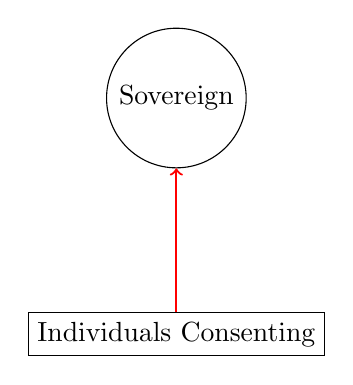
\begin{tikzpicture}
		\path (0,3) node[circle, draw] (A) {Sovereign}
			(0,0) node[rectangle, draw] (B) {Individuals Consenting};
		\draw [<-, thick, red] (A) -- (B);
	\end{tikzpicture}

	Individuals consenting give their rights up to the sovereign which exists outside of the contract. If they existed in the contract, the sovereign would not be absolute.
\end{center}

\subsubsection{Dilemma 1: Reckoning with Laws of Nature}
There is a question about the requirement for the Laws of Nature (LoN) for Hobbes. Previous arguments have shown that these LoN have provided the impetus for consenting into the sovereign. However, we can now question to what extent that is true. In some sense, we can use these laws to show the natural human instinct to shift out of the state of war but in another sense, it may not be the desire for peace but rather a desire to avoid premature death that catalyses the need for government. Hobbes himself even mentions the idea of reasoning as reckoning, this makes it all the more difficult to consolidate our knowledge of human motivation with the moral language of these LoNs.

Yet, if we base it all on self-interest, is there an acknowledgement of moral obligations? The question remains that maybe the LoN are required to have some sort of language that we can use to bind ourselves to a contractual agreement. This is especially important when we contract ourselves to the sovereign.

\subsubsection{Dilemma 2: Authors, Actors and Agents, Hobbes on Representation}
We first question: what is the justification to absolute rule? Hobbes states that there is a justification through \textbf{self interest} whereby the sovereign is required to avoid calamity amongst individuals. Hence, we contract to obligate, this is a necessarily voluntary process because it is in our interests i.e. there is \textbf{no natural obligation} to the ruler.

Yet, if subjects are authors of their own subjection and the sovereign represents the subjects, are the subjects not the sovereign? This presents an issue of responsibility whereby it seems that these subjects are, yet again, responsible for themselves.

Before we go any further, here is some terminology on types of persons:
\begin{itemize}
	\item Natural Persons: people themselves
	\item Artificial Persons: an entity acting in the name of another
\end{itemize}
Hence, the state and sovereign is an artificial person whose words and actions are owned by those who they represent. \textbf{This is to say that the natural person is the author of the leviathan.} Thus, if the actor acts against the Laws of Nature, the author is in the wrong due to the representation process we have just identified. Yet, in this relationship \textbf{you are also a subject in this relationship:}
\begin{itemize}
	\item You are to blame but cannot do anything to fix the situation
	\item If you attempt to fix the situation, you breach your own contract
\end{itemize}
So it looks as if the individual is stuck in this odd and contradictory relationship as either:
\begin{itemize}
	\item Authors (contracting subjects) are responsible for the actor's (sovereign's) wrongs, in which case they must be able to break their contract with it
	\item OR, authors cannot break the contract with the actor, in which case they are not responsible for the actor's ways.
\end{itemize}
You simply cannot have both.

\subsubsection{Limits of Political Obligation}
Remembering that we justify the absolute sovereign through consent and only so far as the sovereign provides protection for its subjects, we can now begin to identify limits to legitimate rule:
\begin{itemize}
	\item A sovereign cannot expect that a person \textit{justly} condemned to death will not defend himself, as there is a legitimate right to self-preservation being breached by the sovereign
	\item A sovereign cannot demand that a person kill another for reasons not for the good of the state
	\item A sovereign cannot ask men of 'feminine courage' or cowardice to fight in the army
\end{itemize}
Hence, we question, \textbf{how far-reaching are these limits?}
\begin{itemize}
	\item Is it in extremis i.e near the point of death)
	\item Can we do it in anticipation and be preemptive about it, like in the SoN
\end{itemize}
So, we can use Hobbes' point of a readiness for war against him. This is because of the idea that if the state looks to be turning against the subject, individuals can preemptively react first against the state before they are harmed. Anticipation as the best form of defence would be the intuitive argument in this scenario.

The subjective perspective on what might seem to be the sovereign working to undermine subjects opens the field of discarding obligation to be very, very wide. Originally, this idea of throwing away obligation seemed slender as we took the point \textbf{in extremis} but now, the scope has been blown open by the way in which we interpret a government's actions, whether they are for or against us.

The essential question that Hobbes needs to answer is why do you distrust your neighbour but not distrust the sovereign? Perhaps it is a qualitatively different entity which is not caught up in the conflicts individuals are concerned with. However, it is built from these contracting peoples and there might still be ground to be skeptical.

Hence, political obligation and its limits is a tough issue for Hobbes. It is entirely dependent on an individual's perspective on the states actions. The state must be very careful not to offend their subjects or encroach upon their security. This is a difficult task to fulfil.

\subsubsection{Hobbes Genius}
We conclude our summaries by understanding Hobbes' Genius:
\begin{itemize}
	\item He made the first conception of the state as an artificial agent distinct from rulers and subjects alike
	\item He articulated a systematic idea of government by consent through the social contract
	\item He had the first modern formulation of the collective action problem through a highly reductive account of human nature and rationality along with this idea of reasoning as reckoning
\end{itemize}

\subsection{Part 2: Study Questions and Plans}
Below are study questions and short, planned responses to them.
\subsubsection{Actors and Agents}
\textbf{Question:} Is Hobbes a democrat despite himself?\\\\
Hobbes initially distinguishes between natural persons and artificial persons when he constructs the social contract. Below is a reminder of what these two things are (Leviathan XVI):
\begin{itemize}
	\item \textbf{A Natural Person} acts as his or her own, his/her own wards and actions are necessarily his/hers
	\item \textbf{A Artificial Person} simply represents the words of others, an entity that is not a person of itself
\end{itemize}
Hence, we recognise that subjects are, themselves, natural persons, while the state or sovereign is, itself, an artificial person representing these subjects.\\\\
\textbf{What it means to be a democrat}\\
To answer this question, we need to define the scope of what it means to be a democrat before considering whether or not Hobbes is a democrat despite himself. There are two key things I believe are essential to this argument:
\begin{itemize}
	\item Principles of Democracy $\rightarrow$ necessary but insufficient conditions of being a democrat
	\item Values of Democracy $\rightarrow$ possibly sufficient conditions of being a democrat
\end{itemize}
From the above, we can deduce that Hobbes might have principles but not be a democrat, have values and be a democrat, or have both and be a democrat. I argue that although Hobbes has the principles, such as actor and agent representation, I do not believe he has the sufficient values, that is to say, that he desires a representative government. Hence, this section will go against the question and argue that Hobbes is not a democrat despite himself.\\\\
\textbf{Hobbes as a principled Democrat}\\
We will go through these two key ideas first to see how they stack up against one another. The principles of Democracy can be distilled into representation and an ability to change that representation based on shifting values and so on. Hobbes supports that to a very large extent, he believes that the artificial superpower of the sovereign has to represent its peoples interests and he makes the initial assumption that peace is in the interests of all consenting individuals. Intuitively, we can see why some would argue that this translates into the idea that Hobbes believes in representation in a democratic context. To that extent, the argument that Hobbes has the necessary conditions to be a democrat is entirely plausible.

Further, the idea that Hobbes proposes, that government is entirely derivative of the people, through our consenting and contracting, shows a strong democratic foundation. Government, it seems, is power to the people. It is distinct from other types of government such as kingship because the sovereign is an abstract entity like the state in a democracy that has a purpose built entirely for its people.

Hence, the agent and actor model shows principles inherent in the democratic model. It is the principle of representation of a people that Hobbes shows which may be related to the democratic idea.\\\\
\textbf{Hobbes lack of Democratic Value}\\
Yet, despite having the necessary conditions, it does not mean that Hobbes has the necessary and sufficient values of being a democrat. This comes from his intentions of the sovereign as a solution to the State of Nature and his assumptions of human motivation.

Hobbes decides that a united will is required for the sovereign. It seems intuitively opposed to a democracy's plethora of views that individuals hold. This means that there needs to be a single guidance that all individuals consent to and that a sovereign itself should not be listening to shifting values and so on. Hobbes distills this by promoting aristocracy or monarchy as ideal types of sovereigns which form a united will in direction but still with the sole purpose of protection.

Further, the Hobbesian assumption of human motivation as driven to find peace might show his understanding of intent as fixated on finding a government fit for the sole purpose of protection. I do not think that democracy is built that way and practical examples, such as voting for gay marriage or less taxation, adds a dimension that Hobbes would not consider as prioritised examples in his sovereign. This shows that the intention that Hobbes is moving forward with is not aligned, in terms of values, with democracy. This, however, might simply be a fault of his assumption and his Laws of Nature. Perhaps, if that were to change, he might have an entirely different view.\\\\
\textbf{Evaluation}\\
From an evaluative standpoint, it is easy to see why the Hobbesian model of agent and actor representation can be conflated with democratic ideals. We have some sort of consent in contracting along with a representation of those people contracting.

However, as I have argued, it is definitely not the Hobbesian intention of being a democrat, even despite himself, and that is due to his lack of the necessary and sufficient values required to be one. His assumptions of human motivation and further, his singular purpose of the sovereign deviates from the typical ideals that democracy promotes. Perhaps for a entire group of individuals seeking peace, it might be representative, but in reality, that might be overly charitable to those believing Hobbes is a democrat.

Although it might seem that he does stumble a little despite himself, I do believe his values are aligned elsewhere and one cannot say that, despite these values, he is democratic as to be democratic, these values are an absolutely necessary condition.

\subsubsection{Political Obligation and Disobedience}
\textbf{Question:} Under what circumstances does Hobbes countenance political disobedience? What does the fact that he countenances it at all imply for his defence of absolute government?\\\\
\textbf{Circumstances}\\
We will begin with the circumstances in which Hobbes allows for political disobedience. Hobbes is only concerned with the state's threats to people's lives and their subsequent right to self-preservation. The only acceptable premise for political disobedience is if \textbf{individual's rights to self-preservation are threatened} in one way or another.

Although we recognise that we consent into an absolute government, it is only absolute in the sense of making decisions related to the protection of its subjects. Hobbes still believes that an individual's right to self-defense is superior to even the absolute's power. Below, we list again, examples of times where political disobedience is permissible:
\begin{itemize}
	\item Being sentenced to death $\rightarrow$ you are no longer under the obligation of the sovereign
	\item Killing with reason $\rightarrow$ if it is not in the interest of the state, it cannot be done, and even if it is in the interest of the state, refer back to previous point
	\item Men of cowardice $\rightarrow$ you cannot be conscripted to go to war
\end{itemize}
The issue with these circumstances is the subjective experience of it. Hence, an individual might preemptively believe that the sovereign will sentence them to death. Does this preemptive belief make legitimate political disobedience? If we recognise Hobbes' idea of preemptive attack or a constant readiness for war as seen in the State of Nature, it would make sense to transfer that logic into the state. Although we have consented to the state and given our rights up to it, it does not mean that we can trust it at all times, especially from an individualistic perspective.

Moreover, with its absolute and unquestionable authority, we begin skeptical again and do not lose that sense of diffidence. It is only the fact that interactions with other people are without conflict, due to the state, that we remain in a peaceful state. If the sovereign happens to misstep, we can begin to question heavily their duty, responsibility and possibly dubious intentions.

Hence, it would seem legitimate if we apply Hobbesian logic that we preemptively move against the state if they are looking to sentence us to death, kill us without reason or even conscript us to the army to fight a war.\\\\
\textbf{Implications}\\
First and foremost, we question the sovereigns power and its extent over its subjects as a result of this broadened scope of political obligation. It seems that the power relation here is not entirely in the hands of the sovereign anymore, rather, real power is in the hands of the individual who can choose when to politically disobey if their subjective perspective on potential harm is made apparent.

Hence, the threat to life in the moment i.e. \textit{in extremis} or foreseeing this threat much further down the line \textit{ex-ante} can catapult the relationship between the individual and sovereign into conflict. The causes of conflict in the State of Nature, especially diffidence, have simply just been translated into the relationship between individual and sovereign rather than individual and state. The question Hobbes might not have answered is how we solve this diffidence between state and individual.\\\\
\textbf{Auxiliary Arguments}\\
\textbf{Eleanor Curran 2005} extends this argument further by discussing the full \textbf{Right to Self-preservation.} She believes that this right is a right to full preservation and is a protected right rather than a claim type of right. That is to say that this right is not access to something but protection from something at all costs. She believes that it is not correlated with the sovereign's duties but is \textbf{protected by the sovereign} to fulfil its office. If it is not, then there is no political obligation.

Further, she labels this as a liberty as there is no obligation to a particular normative claim, all excesses are permitted if one can justify it in accordance to this liberty. It is not a law as that has an obligation to a particular normative claim, like Hobbes stating that humans are motivated to find peace.

But a more interesting twist that Curran puts on this right goes beyond just the preservation of body and limbs, death and pain. She states that full preservation is about protecting oneself from being \textbf{weary of life.} Here, there is a lot of subjectivity and interpretation but the general idea involves living a commodious life which is retained in the commonwealth. This means engaging in leisure, industry and relationships which provides some sense of flourishing outside of just \textbf{protection.} You might be able to argue that the Hobbesian conception of a sovereign does not really provide this. \textbf{n.b. This fits well with the democracy and representation argument too!}

Hence the role of the sovereign is to simply protect this right to full preservation. One could say that there is a \textbf{moral duty} and a \textbf{requirement of office} that the sovereign must fulfil to remain legitimate and it pertains to this particular liberty.

\textbf{Jean Hampton 1987} adds to this argument as she states that the absolute sovereign fails entirely with gaps in its duties. This is because it makes the subjects the judges of whether or not they obey the sovereign's laws due to this issue of subjectivity. Thus the sovereign, in a sense, is really invalid in its ability to conduct its operation of maintaining the peace as it really has no authority and cannot fulfil its proposed duty.

\textbf{Conal Condren (2000) and Edwin Curley (1994)} augment this even further by stating how individuals submit themselves to the sovereign only for security. If security is not had, we cannot say that we have submitted to anything in the first place since security and peace is the critical condition, their proposed counter case is a submission into self-destruction. But since the subject gets to decide whether protection is given or not, there is the issue of \textbf{subjectivity} once more. This shows the true power allocation between the Hobbesian sovereign and the consenting individual.\\\\
\textbf{Evaluation}\\
For Hobbes, political obligation is a particularly pernicious subject since there are many traps, which the individual in society can lay, which might catch out the sovereign.

Perhaps some of the arguments we have levelled against Hobbes might be uncharitable in the sense that Hobbes would give good reason for an absolute sovereign to act within reasonable boundaries even when an individual is skeptical of the sovereign's actions.

Yet, it does seem more intuitive that an individual has the liberty to act, especially with the Hobbesian idea that this right to full self-preservation is supreme over all other rights. I believe that political obligation is an unresolved dilemma that Hobbes faced and a study into understanding the authority that is given, the extents and limits and how they interact with different individuals with differing perspectives would be another topic for another time.


\subsection{Past Paper Questions:}
\begin{itemize}
	\item While Hobbes offers us a realistic portrait of the human condition, his solution to the problem is simplistic and naive. Discuss.
	\item Some critics have argued that the inhabitants of Hobbes' state of nature would never be able to find a way out of it. Is this true, and if it is true, is it a problem for Hobbes?
	\item Hobbes cared about order, but not about justice or freedom. Discuss
\end{itemize}

\subsubsection{Human Condition and Solutions}
\textbf{Question:} While Hobbes offers us a realistic portrait of the human condition, his solution to the problem is simplistic and naive. Discuss. \\\\
\textbf{The Human Condition:}\\
\textbf{Supporting Hobbes}
\begin{itemize}
	\item Legitimate due to Ring of Gyges - Glaucon Example, illuminates our own motivations
	\item Why do we lock our doors after leaving our houses?
	\item Intuitively skeptical of human motivation
	\item Empirical examples of conflict as a result of no order leading to the human condition in a perpetual state of nature
	\item Rationalisation of behaviour that leads to us believing that it is rational to go to war or be ready for it		
	\item Referencing the three principles of conflict: competition, glory and diffidence
\end{itemize}
\textbf{Against Hobbes}
\begin{itemize}
	\item Argument may be too reductive and intuitively not as holistic
	\item Aristotelian natural associations which do not show this perpetual state of war
	\item Associations go into families and villages, perhaps not so much a state yet but shows aspects of mutual friendly association not reducible to conflict
	\item Competition might not occur in these villages if they are able to transact even without the state
	\item Rational to not go to war in these types of communities (Lloyd and Sreedhar 2018) due to the larger benefit that arises from maintaining this mutual cooperation, does not mean that we are not psychologically egoistic
\end{itemize}
\textbf{Solution is simplistic and naive:}\\\\
\textbf{Against the Solution}


\subsubsection{State of Nature and a Way Out}

\subsubsection{Order over Justice and Freedom}

\subsection{Part 2: Appendix}
Here are some additional resources to aid revision:
\begin{itemize}
	\item \href{https://www.jstor.org/stable/27639430?seq=1#page_scan_tab_contents}{Can Rights Curb the Hobbesian Sovereign? E. Curran 2006}
	\item \href{http://muse.jhu.edu.gate3.library.lse.ac.uk/article/566925}{Authorisation and Political Authority. M. Green 2015}
	\item \href{https://www-cambridge-org.gate3.library.lse.ac.uk/core/books/hobbes-and-the-social-contract-tradition/269668B2323D23C3799CCC84A6A64D66}{Hobbes and the Social Contract Tradition. J. Hampton 1987}
	\item \href{http://muse.jhu.edu.gate3.library.lse.ac.uk/article/37609}{Hobbes on Law, Nature and Reason. K. Hoekstra 2003}

\end{itemize}

\newpage
\section{John Stuart Mill}
We start Mill with discussing his key ideas of liberty and utility before moving onto the wide ideas of social progress that he adopts in his later thinking.

\subsection{Part 1: Utility and Liberty}
Mill's thought is borne from the idea that we are naturally the type of being that develops its abilities which is a naturalistic tradition of thinking. This is similar to the Aristotelian line of thought. However, Bentham, a good friend of Mill's father, had a great influence on Mill's early education with its secular line of thought. What Mill seeks to resolve is the diametric opposition between utility and liberty.

This crisis was due to his fall out with romantic poetry whereby he discovers a yearning for individual development.

\subsubsection{Bentham and Beneficic Calculus}
To gain an understanding of liberty, we will first look at the basics of Bentham's Utilitarianism. The basic premises are as follows:
\begin{itemize}
	\item Everyone counts for one and no more than one
	\item The aim of morality is to maximise the greatest possible happiness for the greatest possible number
	\item The aim of the model is to maximise the happiness for the greatest possible number
	\item Happiness is pleasure and the absence of pain - a hedonistic conception of happiness
	\item Utilitarianism counts \textbf{units of happiness} thus \textbf{intensity of preference} along with \textbf{quantity} are equally as important
\end{itemize}
Since we are only interested in aggregate well-being, we are not so much interested in individual well-being. Hence, discounting of individuals would be acceptable under the Bentham calculus. This assignment of all individuals to one unit shows a strong egalitarian argument.

Happiness for Bentham is related to this freedom for hunger, cold, disease and social misery. It is unlike Aristotle's Virtue of Flourishing. He thinks about the basic needs such as a roof over one's head and food for one's stomach.

Utilitarianism is about maximising as much \textbf{utility} as you can. It does not take into account rights which are \textit{nonsense upon stilts} but rather quantifiable levels of happiness. Obviously, the measure is very tough and many arguments could be levelled against Bentham's calculus

\subsubsection{Mill's Modification of Utilitarianism}
Mill endorses the utilitarian view that those actions are good which contribute to human happiness; however, he operates with a less hedonistic conception of happiness. Mill rejects the idea that individual happiness can be \textbf{legitimately sacrificed to social happiness} as social happiness is a function of individual happiness i.e. \textbf{society advances when individual members flourish.}

It is much less hedonistic but more demanding on individual's actions. It rejects the calculus and is a sort of rule-based utilitarianism rather than act-based in a Bentham sense. Below is a key summary of his similarities and differences:
\begin{itemize}
	\item Pleasure and freedom from pain are the only things that are desirable as ends
	\item However, pushpin \textbf{is not as good as} poetry for Mill
	\item There should be a distinction between higher and lower pleasures
	\item This is due to human beings having higher faculties than human appetites
\end{itemize}
Mill believes that we are interested more in the higher pleasures than lower pleasures. Thus, some pursuits are more worthwhile than others, it is a qualitative rather than quantitative notion. Man is supposed to be thought of as a progressive being, similar to Aristotle and his Acorn. Man comes into the world with potential and if we do not structure ourselves properly, we will not be able to develop this potential.

\subsubsection{Social Utility of Individual Liberty}
Mill was also concerned with the tyranny of the majority where the effects of mass conformity and mass society will keep overruling individual self-development. Social progress would not be possible if the masses are against it. There are two key threats to individual liberty that Mill recognises:
\begin{itemize}
	\item \textbf{Governmental/Legal Paternalism:} the prohibition or repression by law of particular types of activity or view, supposedly for people's own good (e.g. marriage laws)
	\item \textbf{Social Repression:} the repressive influence of custom and majority opinion on individual development and flourishing
\end{itemize}
A key idea for Mill is his Harm principle:
\begin{center}
	\fbox{\begin{minipage}{.8\textwidth}
			\begin{center}	
			A bulwark against Government intrusion into individual lives:\\\\
				\textit{The sole end for which mankind are warranted, individually or collectively, in interfering with the liberty of action of any of their number, is self-protection.
				The only purpose for which power can be rightfully exercised over any member of a civilised community, against his will, \textbf{is to prevent harm to others} ... Over himself, over his own body and mind, \textbf{the individual is sovereign.}}
			\end{center}
	\end{minipage}}
\end{center}
One should be allowed to do anything they want insofar as their actions do not harm others. It is a private and public split whereby the private should not be interfered with by others and, above all, the government. This is individual liberty for the sake for the individuals. However, it does not make a case for the \textbf{social usefulness for liberty.}\\\\
Mill also is an adamant supporter of \textbf{free speech} because of its benefits to social progress. The mental well-being of mankind depends on freedom of opinion and freedom of expression on four grounds:
\begin{itemize}
	\item If any opinion is compelled to silence, that opinion may for all we know, be true. \textbf{Silencing of this opinion is not socially useful especially if it's true}
	\item Even if it is in error, it may, and commonly does contain a portion of the truth - \textbf{only the collision of adverse opinions advances truth}
	\item Unless they are vigorously discussed and debated, received opinions, \textbf{even though true, will be dogmas}
	\item Unless debated and discussed, the meaning of true doctrines will be enfeebled
\end{itemize}
Mill also tolerates \textbf{experiments in living}
\begin{itemize}
	\item Not wearing down into uniformity all that is individual in themselves
	\item About cultivation and calling forth, within the limits of rights, that human beings become noble and beautiful
	\item Mill states: \textbf{The imitation of all wise and noble things comes and must come from individuals; generally at first from some one individual}
	\item This shows a social utility from allowing individuals to \textbf{flourish}
\end{itemize}

\subsubsection{Assessing Mill's Arguments}
\textbf{Mill's Defense of Individual Liberty}\\
Mill defends individual liberty for social utility, but what if it's not socially useful?
Mill sees it as important to human flourishing, however, he defends it on grounds of its conduciveness to social progress and his arguments for it seems to be not so convincing.

If individual liberty is to be defended on grounds of its contribution of social progress, \textbf{should we cease to defend it whenever it turns out not to be conducive to social progress?} Another question is: \textbf{are all exercises of individual liberty inherently conducive to social progress?}\\\\
\textbf{Mill's Conception of Pleasure}\\
Mill's split of higher and lower pleasures and leans towards the higher pleasures, is he not elitist? Is he defending liberty at all if one desires to pursue lower pleasures? Is liberty worth anything if not pursuing higher liberties?

Should one who is at liberty to do as he pleases not be free to pursue the lower pleasures? If these are not conducive to social progress, should he be prohibited from pursuing them? The question remains: \textbf{is Mill after social progress or individual liberty? It seems that they are not fully compatible.} Liberty might not be worth having if you are pursuing low pleasures for Mill.\\\\
\textbf{Mill's Harm Principle}\\
The big question for Mill is what harm is. Physical harm? Psychological harm? Foreseeable harm or unforeseeable harm? There is a lot of room for interpretation here.
\begin{itemize}
	\item \textbf{Physical:} don't commit actions that directly injure others
	\item \textbf{Psychological:} don't engage in activities that offend some people
	\item \textbf{Foreseeable Harm:} don't do things that will predictably harm others
	\item \textbf{Unforeseeable Harm:} don't commit actions that may or may not harm others in some ways further down the line
\end{itemize}
The harm principle may become very restrictive, Mill's conception is very vague.\\\\
\textbf{Mill and Self-Regarding action}\\
There are some trivial acts that might not be all about individual sovereignty:
\begin{itemize}
	\item Watching pornography
	\item Abortion as a private choice
	\item University and getting a degree
\end{itemize}
Do these require industries to be at one's service? Are there any private choices at all? This distinction between the private and public is crucial to liberalism because there are areas where the government should not interfere.

Hence, the distinction is always contested. Perhaps this is a strength of Mill, where everything is up for negotiation and there is a progress behind them. Hence the vagueness is the strength. The worst thing would be to stop arguing about these divisions. 


\subsection{Part 1: Study Questions and Plans}
Below are study questions and short, planned responses to them.

\subsubsection{Progressive Beings}
\textbf{Question:} What does Mill mean when he speaks of man as a progressive being? How does Mill's conception of human happiness and flourishing compare with Aristotle's notion of human flourishing in terms of the practice of virtue?\\\\
The progressive being is Mill's idea of how individuals are born with natural faculties which have the potential to be developed. It is argued in a romantic sense where Mill believes that individuals all have different natures and must be given space to discover and develop their own personalities and ways of living.

Mill states that: \textbf{Human nature is not a machine to be built after a model, and set to do exactly the work prescribed for it, but a tree, which requires to grow and develop itself on all sides, according to the tendency of the inward forces which make it a living thing.} Hence, there is the critical idea of a free type of growth.\\\\
\textbf{Progressive Being}
So we being by defining some key features of the progressive being:
\begin{itemize}
	\item Individuals are all diverse and different natured
	\item Individuals each have their own natural faculties with potential to be developed
	\item Individuals choose their lives for oneself
	\item Hence, individuals \textbf{progress} by conducting their own experiments of living
\end{itemize}
The idea associated with this experiment of living is to allow for a plethora of ways of living to essentially coexist with one another. This is because a diversity of character and culture, to Mill, provides the end of \textit{productive tension} that drives a nation forward. Without this tension, there would be a stationariness which would mean accepting principles as they are with no contest.
\\\\
\textbf{Comparison with Aristotle}\\
The second part of the question requires an understanding of Aristotelian virtue and flourishing towards Eudaimonia along with recognising the differences that Mill might have to this virtue ethic.

\textbf{Aristotle's} virtue ethic and form of human flourishing is following the ideal man. This is based on how one cultivates their virtues and grows them in tandem with growing their own person. For Aristotle, there is a need for \textit{phronesis} which can be understood as practical wisdom.
This is the idea that to develop, one must be able to learn practically and apply practically.

Virtues such as moderation, courage and wisdom are all examples of the flourishing individual for Aristotle. Note that all of these virtues are in between two vices, courage is between timidness and foolhardiness for example.
\\\\
\textbf{Mill's} idea of happiness and flourishing is similar to a certain extent. One of the critical similarities is the practical aspect of virtue for Aristotle and for Mill. Phronesis, in Mill's theory is through these experiments of living where we recognise the testing and reconfiguring of each individual's path to flourishing.

Further, Mill does provide a goal to work towards which he defines as the higher pleasures. This is similar to Aristotle in the sense that there is an ideal configuration of pleasures that humans should work towards in their experiments of living. Further, the ideal configuration with Aristotle as well as Mill encompasses a lot of possibilities in what type of person you could be. That is to say, there is flexibility in the argument where there are multiple higher pleasures one can adopt to flourish as well as a rigidity whereby one must be adopting these higher pleasures or virtues.
\\\\
\textbf{Against Aristotle}\\
Yet, Mill's arguments for happiness and human flourishing, despite the previous rigidity mentioned, be a bit less strict than the fully ideal human that Aristotle advocates for. I argue that Mill's progressive being is not as perfect or does not strive to be as perfect as the Aristotelian eudaimon.

The one main reason for this difference is due to the \textbf{continuous change} that Mill advocates for. I do not think that there is a particular endpoint that Mill has in mind but that progress continuously reshapes the endpoints that individuals strive towards. For Aristotle, I do not think that is the case as there is one particular configuration of virtue that makes the man. Although these sets of virtues are adaptable to all situations, the virtues remain the same.

For Mill, it is hard to argue that the virtues, bar the principle of liberty, remains totally constant as experiments of living, especially in a private sense, can extend beyond the Aristotelian limits of virtue as long as they do not harm others. For Aristotle, this would seem absurd and not really key to the concept of phronesis. This is because the virtue's golden mean would be spoilt by such experiments which deviate heavily from the norm.

Mill would still argue that irrespective of what activity one undertakes, progress is somehow being made. Hence, perhaps it goes beyond perfection whereby the definition of perfect is reshaped with each experiment. Otherwise, one might not be striving for perfection at all but to continuously learn and keep reshaping in a Mill sort of way.
\\\\
\textbf{Evaluation}\\
Thus, to a certain extent, the progressive being is similar to the Aristotelian Eudaimon. Individuals practice and experiment to approach a type of flourishing that allows them to progress and develop as people. There are certain sets of pleasures for Mill and certain virtues for Aristotle that show that an individual has flourished.

However, Mill goes beyond the Aristotelian point of perfection to continuously experiment. Even with higher pleasures already allocated by Mill, there is still a belief that contradictions and arguments about what is right or wrong are essential irrespective of what Mill, himself, believes. Hence, his theory goes beyond himself to allow for a certain expandability on what type of pleasure we should strive towards to progress. It certainly moves beyond Aristotle's virtue to a very large extent.


\subsubsection{Liberty and Social Utility}
\textbf{Question:} Does Mill succeed in showing that the pursuit of individual liberty is socially useful, or would he have done better defending individual liberty on its own terms?\\\\
Mill's argument for individually liberty is based on four critical premises:
\begin{itemize}
	\item Opinions which are compelled to silence may be true
	\item Opinions which are errors commonly have a portion of truth
	\item Opinions should be continuously discussed so that none of them become dogmas
	\item Opinions should be discussed so as to reinforce their meaning otherwise their meaning may be lost
\end{itemize}
Hence, we can recognise that the liberty to express oneself, with the above four ideas related to freedom of speech, is absolutely critical to society. This is to ensure that society is consistently learning from one another even if one opinion will ultimately be overrided by another.

The toleration of experiments in living adds to this idea of social progress. Mill is ultimately afraid of wearing down individuals into uniformity. Mill, rather, is concerned about flourishing and the cultivation of individual's potentials which is similar to an Aristotelian virtue approach as discussed above. Therefore the use of this to society is through a constant re-evaluation of virtue that adds to a knowledge base in society but also allows for the whole of society, built of individuals, to flourish in their respective domains simultaneously. Thus, liberty is not valuable in itself, but as the most reliable means of producing something else that would be seen as valuable.

Returning to our list, we can pick apart each concept to see how the freedom of expression is useful to society:
\begin{itemize}
	\item \textbf{Silenced Truth:} this one is not hard to intuitively understand. Truth, which is kept silent, does not add any value whatsoever to society. Freedom of expression, to a large extent, allows for this truth to come out and be talked about. This adds utility to society as everyone would be able to gain knowledge of this truth. Whether or not it is true is another question.
	\item \textbf{Portions of Truth:} this is another addition to truth and the discourse that would arise as a result of debating what is right and wrong and in which contexts will also prove to be fruitful for society. This is because knowledge is further gained and no single individual is suppressed.
	\item \textbf{Stopping Dogma:} this one is perhaps trickier to level with someone like Plato who would advocate for strong dogma, like the craft analogy and noble lie, to institute a well ordered and just city. However, our liberal perspectives would argue that individuals should be able to pursue their own experiments in living and dogma would not be conducive to that. Although there might be some absolute and certain truths, it remains that other concepts and ideas that might be taken for granted or taken as a given subconsciously, should be challenged as well.
	\item \textbf{Reinforcing Meaning:} discussion to reinforce meaning adds utility by ensuring that we have things as ordered as they should be. Meaning which is lost would result in a net negative to society as individuals would not understand the way in which such ideas or concepts come about. This links back to the dogma idea but instead of dogma, concepts are just taken for granted instead.
\end{itemize}
Thus, from above, we can recognise the importance Mill's liberty has for society and why he argues for its instrumental use rather than arguing that it is a good in itself alone. Mill adamantly believes that the mental well-being of mankind depends on this freedom of opinion and expression.
\\\\
\textbf{Do all acts of liberty aid society?}
\\
Not necessarily and this is an argument that Mill needs to level with his defence of liberty through its utility. The defence of liberty alone will be discussed below.

To say that all acts of liberty are conducive to society would be a counter-intuitive exercise. Mill mentions that even wrong acts have some portion of truth that might be helpful for society to progress. That can be taken seriously to a certain extent, but how far? Perhaps certain individual actions and experiments of living as trivial as hurting oneself by accidentally hitting your thumb with a hammer might not be conducive to social progress.

Although one could argue that this is done without intention, one can counter that many assumed wrong acts are. This breadth that Mill adopts almost seems to large and wide that it'd become counter-intuitive. Acts which we question as stupid, pointless and meaningless, acts which we deem trivial and others deem experiments of living might not have the effect Mill intended.
\\\\
\textbf{How do all acts matter?}
\\
Perhaps more exploration on why all acts matter should be done. Mill's argument arises from portions of truth but perhaps a way of rephrasing this is understanding all acts as lessons. Lessons for things to do and what not to do, whether or not these acts constitute higher or lower pleasures.

Taking our examples of stupid and pointless acts, perhaps a Mill type of response would be to see these as acts not to undertake in the future. Any further iteration of this act would be a reminder of this truth, referring to the fourth principle, as to promote discussion and debate on why such an act would be pointless or stupid.

Although this might seem directionless for these bizarre acts, we can still adopt an optimism when looking at these experiments to learn something. For Mill, perhaps that small something is what gives it value.
\\\\
\textbf{Liberty Defended Alone}\\
The question asks if liberty should be defended alone. I do not know if Mill's arguments and \textbf{further defending Liberty alone} would be mutually exclusive. It could be the case that they could reinforce one another. However, let us explore the case of defending liberty alone first.

Perhaps the idea here is that the case for social utility as a defence for liberty is not holistic enough and so Mill should embark on two separate journeys to defend experiments of living for their social utility but not defend liberty for an instrumental purpose.

Thus, the argument that liberty should be defended as a good in itself rather than a means to an ends should be recognised as the better alternative. This means we defend liberty because it is simply a concept that must be defended. It is intrinsic to our nature and immutable hence any threat to it should be taken seriously.

Many other theorists would defend liberty in this way with a concept of right or even a Hobbesian concept of self-preservation thus the argument for liberty itself should be handled elsewhere. We will now further explore whether or not Mill's claims for social utility are sufficient enough.

I argue that social utility as a defence for liberty should be used to reinforce liberty's own intrinsic value. That is, liberty is good in itself and good for social liberty but one should not argue that social utility is the only justification for liberty. That would lead to a lot of difficult circles to square.

The social utility aspect, especially with regards to experiments for living, should definitely aid in understanding why liberty is so important and useful to defend in society. These arguments have already been detailed above and definitely show an intuitive response, perhaps due to our liberal disposition, to why we allocate so much importance to liberty.

The difficulty is to see how liberty matches with social utility in times when liberty is a hindrance, this would be a very Bentham type of calculus whereby the quantitative approach of utility appears to have a much cleaner answer than the Mill qualitative type. Here is where the defence of liberty alone needs to be fully realised.
\\\\
\textbf{Evaluation}
\\
For Mill, perhaps more work to defending liberty alone should be done to reinforce his argument. The defence from social utility does not stand its own ground due to the breadth it covers whereby liberty may come to be a hindrance rather than an aid to social circumstances.

Hence, look at utility as reinforcement for liberty for the most part, however, when liberty confronts utility, a defence of liberty alone is critical to Mill's argument's success.


\subsubsection{Harm Principle}
\textbf{Question:} What is the harm principle? Is it a good guide to individual conduct within the constraints of social living? Is Mill right to insist on the harm principle as the sole ground of governmental restriction of individual liberty?





\subsection{Part 1: Appendix}



\subsection{Part 2: Social Progress}

\subsection{Part 2: Study Questions and Plans}

\subsection{Part 2: Appendix}



\newpage
\section{Kwame Nkrumah}



\end{document}
